%% History:
% Pavel Tvrdik (26.12.2004)
%  + initial version for PhD Report
%
% Daniel Sykora (27.01.2005)
%
% Michal Valenta (3.12.2008)
% rada zmen ve formatovani (diky M. Duškovi, J. Holubovi a J. Žďárkovi)
% sjednoceni zdrojoveho kodu pro anglickou, ceskou, bakalarskou a diplomovou praci

% One-page layout: (proof-)reading on display
%%%% \documentclass[11pt,oneside,a4paper]{book}
% Two-page layout: final printing
\documentclass[11pt,twoside,a4paper]{book}   
%=-=-=-=-=-=-=-=-=-=-=-=--=%
% The user of this template may find useful to have an alternative to these 
% officially suggested packages:
\usepackage[czech, english]{babel}
\usepackage[T1]{fontenc} % pouzije EC fonty 
\usepackage{listings} %pouzivani referencovatelneho bloku kodu 
% pripadne pisete-li cesky, pak lze zkusit take:
% \usepackage[OT1]{fontenc} 
\usepackage[utf8]{inputenc}
%=-=-=-=-=-=-=-=-=-=-=-=--=%
% In case of problems with PDF fonts, one may try to uncomment this line:
%\usepackage{lmodern}
%=-=-=-=-=-=-=-=-=-=-=-=--=%
%=-=-=-=-=-=-=-=-=-=-=-=--=%
% Depending on your particular TeX distribution and version of conversion tools 
% (dvips/dvipdf/ps2pdf), some (advanced | desperate) users may prefer to use 
% different settings.
% Please uncomment the following style and use your CSLaTeX (cslatex/pdfcslatex) 
% to process your work. Note however, this file is in UTF-8 and a conversion to 
% your native encoding may be required. Some settings below depend on babel 
% macros and should also be modified. See \selectlanguage \iflanguage.
%\usepackage{czech}  %%%%%\usepackage[T1]{czech} %%%%[IL2] [T1] [OT1]
%=-=-=-=-=-=-=-=-=-=-=-=--=%

%%%%%%%%%%%%%%%%%%%%%%%%%%%%%%%%%%%%%%%
% Styles required in your work follow %
%%%%%%%%%%%%%%%%%%%%%%%%%%%%%%%%%%%%%%%
\usepackage{graphicx}
%\usepackage{indentfirst} %1. odstavec jako v cestine.
\usepackage{zref-savepos}
\usepackage{k336_thesis_macros} % specialni makra pro formatovani DP a BP
 % muzete si vytvorit i sva vlastni v souboru k336_thesis_macros.sty
 % najdete  radu jednoduchych definic, ktere zde ani nejsou pouzity
 % napriklad: 
 % \newcommand{\bfig}{\begin{figure}\begin{center}}
 % \newcommand{\efig}{\end{center}\end{figure}}
 % umoznuje pouzit prikaz \bfig namisto \begin{figure}\begin{center} atd.

\makeatletter
% \zsaveposx is defined since 2011/12/05 v2.23 of zref-savepos
\@ifundefined{zsaveposx}{\let\zsaveposx\zsavepos}{}
\makeatother
\newcounter{hposcnt}
\renewcommand*{\thehposcnt}{hpos\number\value{hposcnt}}
\newcommand*{\SP}{% set position
  \stepcounter{hposcnt}%
  \zsaveposx{\thehposcnt s}%
}
\makeatletter
\newcommand*{\UP}{% use previous position
  \zsaveposx{\thehposcnt u}%
  \zref@refused{\thehposcnt s}%
  \zref@refused{\thehposcnt u}%
  \kern\zposx{\thehposcnt s}sp\relax
  \kern-\zposx{\thehposcnt u}sp\relax
}
\makeatother


%%%%%%%%%%%%%%%%%%%%%%%%%%%%%%%%%%%%%
% Zvolte jednu z moznosti 
% Choose one of the following options
%%%%%%%%%%%%%%%%%%%%%%%%%%%%%%%%%%%%%
\newcommand\TypeOfWork{Diplomová práce} \typeout{Diplomova prace}
% \newcommand\TypeOfWork{Master's Thesis}   \typeout{Master's Thesis} 
% \newcommand\TypeOfWork{Bakalářská práce}  \typeout{Bakalarska prace}
% \newcommand\TypeOfWork{Bachelor's Project}  \typeout{Bachelor's Project}


%%%%%%%%%%%%%%%%%%%%%%%%%%%%%%%%%%%%%
% Zvolte jednu z moznosti 
% Choose one of the following options
%%%%%%%%%%%%%%%%%%%%%%%%%%%%%%%%%%%%%
% nabidky jsou z: http://www.fel.cvut.cz/cz/education/bk/prehled.html

%\newcommand\StudProgram{Elektrotechnika a informatika, dobíhající, Bakalářský}
%\newcommand\StudProgram{Elektrotechnika a informatika, dobíhající, Magisterský}
% \newcommand\StudProgram{Elektrotechnika a informatika, strukturovaný, Bakalářský}
 \newcommand\StudProgram{Otevřená informatika, strukturovaný,
 Navazující magisterský}
% \newcommand\StudProgram{Softwarové technologie a management, Bakalářský}
% English study:
% \newcommand\StudProgram{Electrical Engineering and Information Technology}  % bachelor programe
% \newcommand\StudProgram{Electrical Engineering and Information Technology}  %master program


%%%%%%%%%%%%%%%%%%%%%%%%%%%%%%%%%%%%%
% Zvolte jednu z moznosti 
% Choose one of the following options
%%%%%%%%%%%%%%%%%%%%%%%%%%%%%%%%%%%%%
% nabidky jsou z: http://www.fel.cvut.cz/cz/education/bk/prehled.html

%\newcommand\StudBranch{Výpočetní technika}   % pro program EaI bak. (dobihajici i strukt.)
\newcommand\StudBranch{Softwarové inženýrství a interakce}   % pro prgoram EaI mag.
% (dobihajici i strukt.) \newcommand\StudBranch{Softwarové inženýrství}            %pro STM
%\newcommand\StudBranch{Web a multimedia}                  % pro STM
%\newcommand\StudBranch{Computer Engineering}              % bachelor programe
%\newcommand\StudBranch{Computer Science and Engineering}  % master programe


%%%%%%%%%%%%%%%%%%%%%%%%%%%%%%%%%%%%%%%%%%%%
% Vyplnte nazev prace, autora a vedouciho
% Set up Work Title, Author and Supervifsor
%%%%%%%%%%%%%%%%%%%%%%%%%%%%%%%%%%%%%%%%%%%%

\newcommand\WorkTitle{Migrace databáze}
\newcommand\FirstandFamilyName{Bc. Martin Lukeš}
\newcommand\Supervisor{Ing. Ondřej Macek}


% Pouzijete-li pdflatex, tak je prijemne, kdyz bude mit vase prace
% funkcni odkazy i v pdf formatu
\usepackage[
pdftitle={\WorkTitle},
pdfauthor={\FirstandFamilyName},
bookmarks=true,
colorlinks=true,
breaklinks=true,
urlcolor=red,
citecolor=blue,
linkcolor=blue,
unicode=true,
]
{hyperref}

\begin{document}

%%%%%%%%%%%%%%%%%%%%%%%%%%%%%%%%%%%%%
% Zvolte jednu z moznosti 
% Choose one of the following options
%%%%%%%%%%%%%%%%%%%%%%%%%%%%%%%%%%%%%
\selectlanguage{czech}
%\selectlanguage{english} 

% prikaz \typeout vypise vyse uvedena nastaveni v prikazovem okne
% pro pohodlne ladeni prace


\iflanguage{czech}{
	 \typeout{************************************************}
	 \typeout{Zvoleny jazyk: cestina}
	 \typeout{Typ prace: \TypeOfWork}
	 \typeout{Studijni program: \StudProgram}
	 \typeout{Obor: \StudBranch}
	 \typeout{Jmeno: \FirstandFamilyName}
	 \typeout{Nazev prace: \WorkTitle}
	 \typeout{Vedouci prace: \Supervisor}
	 \typeout{***************************************************}
	 \newcommand\Department{Katedra počítačů}
	 \newcommand\Faculty{Fakulta elektrotechnická}
	 \newcommand\University{České vysoké učení technické v Praze}
	 \newcommand\labelSupervisor{Vedoucí práce}
	 \newcommand\labelStudProgram{Studijní program}
	 \newcommand\labelStudBranch{Obor}
}{
	 \typeout{************************************************}
	 \typeout{Language: english}
	 \typeout{Type of Work: \TypeOfWork}
	 \typeout{Study Program: \StudProgram}
	 \typeout{Study Branch: \StudBranch}
	 \typeout{Author: \FirstandFamilyName}
	 \typeout{Title: \WorkTitle}
	 \typeout{Supervisor: \Supervisor}
	 \typeout{***************************************************}
	 \newcommand\Department{Department of Computer Science and Engineering}
	 \newcommand\Faculty{Faculty of Electrical Engineering}
	 \newcommand\University{Czech Technical University in Prague}
	 \newcommand\labelSupervisor{Supervisor}
	 \newcommand\labelStudProgram{Study Programme} 
	 \newcommand\labelStudBranch{Field of Study}
}




%%%%%%%%%%%%%%%%%%%%%%%%%%    Poznamky ke kompletaci prace
% Nasledujici pasaz uzavrenou v {} ve sve praci samozrejme 
% zakomentujte nebo odstrante. 
% Ve vysledne svazane praci bude nahrazena skutecnym 
% oficialnim zadanim vasi prace.
{
\pagenumbering{roman} \cleardoublepage \thispagestyle{empty}
\chapter*{Na tomto místě bude oficiální zadání vaší práce}
\begin{itemize}
\item Toto zadání je podepsané děkanem a vedoucím katedry,
\item musíte si ho vyzvednout na studiijním oddělení Katedry počítačů na Karlově náměstí,
\item v jedné odevzdané práci bude originál tohoto zadání (originál zůstává po obhajobě na katedře),
\item ve druhé bude na stejném místě neověřená kopie tohoto dokumentu (tato se vám vrátí po obhajobě).
\end{itemize}
\newpage
}

%%%%%%%%%%%%%%%%%%%%%%%%%%    Titulni stranka / Title page 

\coverpagestarts

%%%%%%%%%%%%%%%%%%%%%%%%%%%    Podekovani / Acknowledgements 

\acknowledgements
\noindent
Chtěl bych poděkovat vedoucímu své diplomové práce Ing. Ondřeji Mackovi za pomoc
s vypracovávánáním této práce. Dále bych chtěl poděkovat svým kolegům z týmu
Migdb, obzvláště Martinu Mazanci, kteří svými připomínkami napomáhali k zkvalitnění této práce a
zahlazení některých nepřesností. V neposlední řadě bych chtěl poděkovat
firmě CollectionsPro s.r.o, jež přišla s původní myšlenkou, která vedla k
vytvoření Migdb týmu.


%%%%%%%%%%%%%%%%%%%%%%%%%%%   Prohlaseni / Declaration 

\declaration{V~Praze dne 22.\,5.\,2014}
%\declaration{In Kořenovice nad Bečvárkou on May 15, 2008}


%%%%%%%%%%%%%%%%%%%%%%%%%%%%    Abstract 
 
\abstractpage
\noindent 
This work is concerned with specifying the contract and implement the transformation changes 
of the application model into changes of the database model. It also
deals with the automation of the derivation of the changes applied to one model
leading to another without loss or with minimal loss of stored data.

% Prace v cestine musi krome abstraktu v anglictine obsahovat i
% abstrakt v cestine.
\vglue60mm

\noindent{\Huge \textbf{Abstrakt}}
\vskip 2.75\baselineskip

\noindent
Tato práce se zabývá upřesněním kontraktu a realizací transformací změn
aplikačního modelu na změny modelu databázového. Dále se zabývá automatizací odvození změn vedoucích z
jednoho modelu k druhému bez ztráty či s minimální ztrátou uložených dat.
%Abstrakt práce by měl velmi stručně vystihovat její podstatu. Tedy čím se práce
% zabývá a co je jejím výsledkem/přínosem.

\noindent
%Očekávají se cca 1 -- 2 odstavce, maximálně půl stránky.

%%%%%%%%%%%%%%%%%%%%%%%%%%%%%%%%  Obsah / Table of Contents 

\tableofcontents


%%%%%%%%%%%%%%%%%%%%%%%%%%%%%%%  Seznam obrazku / List of Figures 

\listoffigures


%%%%%%%%%%%%%%%%%%%%%%%%%%%%%%%  Seznam tabulek / List of Tables

\listoftables


%**************************************************************

\mainbodystarts
% Odsazeni prvniho radku odstavce resi class book (neaplikuje se na prvni 
% odstavce kapitol, sekci, podsekci atd.) Viz usepackage{indentfirst}.
% Chcete-li selektivne zamezit odsazeni 1. radku nektereho odstavce,
% pouzijte prikaz \noindent.

%**************************************************************

% Pro snadnejsi praci s vetsimi texty je rozumne tyto rozdelit
% do samostatnych souboru nejlepe dle kapitol a tyto potom vkladat
% pomoci prikazu \include{jmeno_souboru.tex} nebo \include{jmeno_souboru}.
% Napr.:
% \input{1_uvod.tex}
% \input{2_teorie.tex}
% atd...

%*****************************************************************************
\chapter{Úvod}
\section{Motivace}

V průběhu poslední dekády je vyvíjeno více nového softwaru než kdy předtím a
současně je i stávající software stále více a častěji modifikován, ať už
je to zapříčiněno  existencí rozsáhlého legacy systému, špatného návrhu či
upravovánim funkcionality softwaru. Dá se předpokládat, že díky masivnímu
rozšíření informačních technologií, obzvláště mobilních tento trend nejenže bude
pokračovat, ale bude i dále na vzestupu.

Díky nutnosti zpracování a ukládání velkého množství dat se již od padesátých
let dvacátého století prosazovaly myšlenky vedoucí k vytvoření speciálních
systémů k těmto účelům určeným - tento software se v české odborné literatuře
nazývá systém řízení báze dat (SŘBD). 

Kvůli nutnosti dokumentace a komunikace mezi vývojáři vznikají různé typy
modelů. Objektový model aplikace popisuje strukturu aplikace a je doplněn 
modelem databázovým modelem popisujícím stav databáze. Nejrozšířenějším typem
databáze jsou v nynější době databáze relační, která uspořádává data podle
relařního modelu. Relační model je dle \cite{Relacni_algebra} formální abstrakce
využívající relaci jakožto jediný konstrukt. Relace je uspořádaná n-tice
souvislých dat R(A1:D1, A2:D2, \ldots An:Dn), přičemž "R" je název relace, Ai
jsou názvy atributů a Di jsou k nim přidružené typy. Relační algebra definuje
pomocí relací a integritních omezení strukturu databáze. Dotazovacím aparátem
pro data definovaná pomocí relační algebry je relační algebra. Relační algebra
využívá operátorů $\bigcup$ (sjednocení), $\bigcap$ (průnik),
$\setminus$ (množinový rozdíl), $\times$ (kartézský součin), selekce
značená R($\varphi $) = \{ u | u $\in$ R a  $\varphi(u)$\} a projekce značená
R[C] = { u[C] | u $\in$ R} a operace přirozené spojení T(C) = R * S =\{u |
u[A] $\in$ R a u[B] $\in$ S\}.
\cite{Relacni_algebra} dále definuje relačně úplný jazyk jako takový, který
umožňuje realizovat relační algebru. Takovým jazykem je například jazyk SQL 
(Structured Query Language). Relační databáze implementuje relaci tabulkou, její
atributy Ai jednotlivými sloupci s typy Di. V dotazovacím jazyce SQL nahrazuje
projekci R[a1, \ldots , an] operací SELECT a1, \ldots an FROM R, operaci
selekce R[ a = 1] klauzulí where v dotaze select  SELECT * FROM R WHERE a = 1; 

Aby byla aplikace funkční, je nutné zajistit
konzistenci mezi databázovým a aplikačním modelem.
Tento problém byl již vyřešen a jeho řešení bývá v literatuře nazýváno objektově
relační mapování(ORM) \cite{ORM}. Dnešní implementace ORM jsou schopny nejen
transformovat aplikační model na model databázový, ale také vyjádřit změnu v struktuře
aplikace pomocí skriptů Data definition Language (DDL), podmnožiny jazyka SQL.
Tyto skripty pozmění model databázový tak aby odpovídal modelu aplikačnímu. Tato konzistence je zaručena automatickou
transformací aplikačního modelu na model databázový, což vývojářům softwaru
šetří čas strávený vývojem softwaru.

Problém nastává, jakmile zahrneme do zachování
nejen strukturu dat, ale i samotná data. Změnit strukturu dat a zároveň
transformovat data tak, aby měla stejnou vyjadřovací schopnost jako původní
data - považujme změny aplikačního modelu jako smazání třídy, atributu apod za
změny zachovávající informaci.


\chapter{Projekt Migdb}

Tato dipomová práce byla napsána v rámci projektu Migdb, který vznikl díky
spolupraci akademické sféry se sférou komerční v roce 2011. Komerční sféra byla
v tomto případě zastoupena firmou CollectionsPro, s.r.o (dále jen CP) a
akademická potom Katedrou počítačů fakulty Elektrotechnické na pražském
Českém vysokém učení technickém. Ambiciózním cílem tohoto projektu bylo od
pořátku projektu definování ucelené množiny změn, tj. operací, kterými mohou vývojáři změnit
model aplikace a transformovat tyto změny do spustitelnáho SQL skriptu, který
změní strukturu databáze a přesune data do odpovídajících elementů z modelu
aplikace.

Zabývá se zkoumáním změn aplikačního modelu, jejich popisem a rozpoznáváním změn
vedoucích od jednoho aplikačního modelu vedoucích k druhému. Dále pak dokončuje a upřesňuje
kontrakt takzvaných operací nad aplikačním modelem a popisuje jejich
transformaci na změny modelu databázového a následným vygenerováním SQL příkazů
spustitelných nad relační databází PostgreSQL.

V rámci Migdb bylo v posledních letech vytvořeny a obhájeny 4 bakalářské práce a
2 diplomové práce členů Migdb.

Jednalo se o tyto bakalářské práce - brakalářská práce mé osoby \cite{Lukes},
jež pojednávala o problematice mapování aplikačního modelu na model databázový,
bakalářské práce Jiřího Ježka \cite{Jezek} popisující aplikační model a jeho
transformace, dále bakalářská práce Petra Taranta \cite{Tarant_bp} popisující
databázový model a jeho transformace a poslední bakalářskou prací je
práce popisující testování projektu \cite{Luksch}.

V roce 2014 byla obhájena diplomová práce Petra Taranta \cite{Tarant_dip}
formálně specifikující aplikační operace a diplomová práce Martina Mazance
\cite{Mazanec} definující doménově specifikující jazyk aplikačních operací.

Projekt Migdb byl započat v spolupráci se společností Collections Pro Výsledky
dosavadní práce byly v roce 2012 prezentovány jako case-study na prestižní
modelové konferenci Code Generation 2012 \cite{Cambridge} v Anglickém Cambridge.

\section{Framework Migdb}
	
Tato kapitola je věnována krátkému představní frameworku Migdb. Projekt Migdb se
věnuje evolučním procesem v průběhu vývoje software. Na obr
\ref{fig:mazanma:framework} převzatého z \cite{Mazanec}. Objektová vrstva každé
aplikace je reprezentována jejím modelem obsahujícím entity aplikace. Databázová
vrstva zajišťuje perzistenci obsahuje jednak schéma definující strukturu
databíze a dále potom samotná perzistované instance dat.

Proces evoluce změn v životním cyklu softwaru definoval v práci \cite{Jezek}
následujícně:


\begin{enumerate}\label{framework:jezek_def}
  \item redefinice entit na objektové vrstvě
  \item opětovná tvorba databázového schématu dle redefinovaných entit
  \item sběr potřebných informací pro migraci dat a příprava migračního skriptu
  \item ověření proveditelnosti migračního skriptu
  \item migrace dat
\end{enumerate}

Po bližší analýze potřeb společnosti CP a po ověření nadbytečnosti vrstvy
ověřující proveditelnost migrovaných skriptů byl tento koncept přepracován do
formy \ref{fig:framework:modified}. Na obrázku vidíme aplikační a databázový
metamodel, které jsou ulořeny v souborech s příponou ecore. Instancemi
aplikačního APP metamodelu jsou jednotlivé generace aplikačního modelu. 
Instancemi databázového RDB metamodelu jsou potom generace RDB modelů. Aplikační
i databázové modely jsou uloženy ve formě .xmi souborů.  Změny, které se
provádějí v aplikaci jsou transformovány na databázové operace aplikovatelné na
RDB model. Databázové operace jsou potom transformovány na SQL scripty. V
původní představě byl do frameworku zapojen i exekutor těchto skriptů nad
databází, ale po konzultaci s CP byl vzhledem k znovupoužitelnosti SQL souborů
z frameworku vypuštěn. 

V rámci projektu jsem vytvořil ve své bakalářské práci \cite{Lukes} ORM
transformaci Aplikační struktury na databázovou a následné vygenerování SQL
skriptu vytvářející strukturu aplikace. Tento nástroj není ve frameworku použit
při nasazení, ale byl použit při testování frameworku - viz
kapitola \ref{chapt:testování}. Ve framework Migdb pracují
oproti původní sekvenční představě viz \ref{framework:jezek_def} po částech
sekvenčně. První aplikační operace je aplikována na aplikační model, je
transformována do databáze, kde jsou je její obraz(sekvence databázových
operací) provedena nad databázovým modelem. Po provedení první operace prochází
tímto cyklem druhá operace, potom třetí \ldots

Evoluce na databázové úrovni nemá vliv na tvar vygenerovaných SQL skriptů, ale
po konzultaci s CP jsme usoudili i po zkušenostech z praxe s databází
Postgresql, že evoluce databázového modelu odhalující chyby je užitečným
uspořením času vývojáře, protože aplikace některých SQL skriptů může trvat(a
typicky trvá) delší čas než průběh evoluce RDB modelu a dobrým nahrazením přímé
exekuce SQL skriptů.

\begin{figure}[ht]
\begin{center}
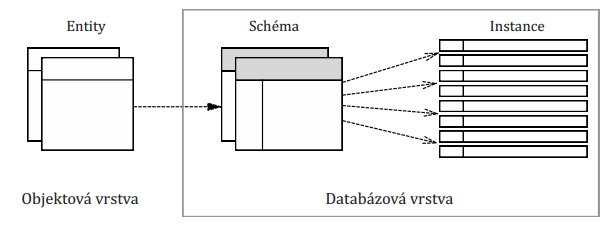
\includegraphics[width=15cm]{figures/framework_structura}
\caption{Rozdělení vrstev softwaru - převzato z \cite{Mazanec}}
\label{fig:mazanma:framework}
\end{center}
\end{figure}


\begin{figure}[ht]
\begin{center}
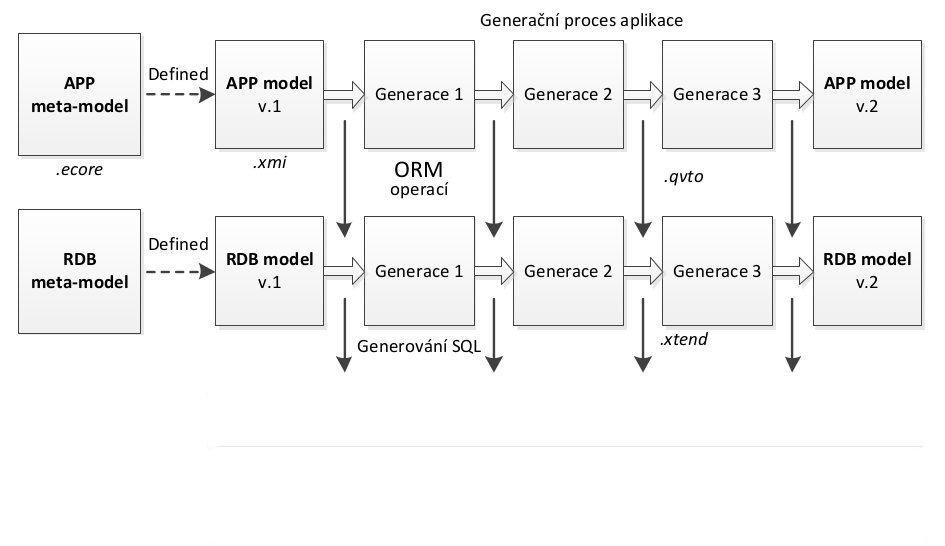
\includegraphics[width=15cm]{figures/framework_structura_tarant_modified}
\caption{Rozdělení vrstev softwaru - převzato z \cite{Tarant_bp} a částečně
upraveno}
\label{fig:framework:modified}
\end{center}
\end{figure}


\section{Aplikační metamodel}

Aplikační model zachycuje vztahy mezi jednotlivými objekty tvořícími
aplikaci. Ačkoliv byl tento model vytvořen již v raných fázích projektu Migdb a
byl často upravován, většinou zjednodušován. Na obrázku \ref{fig:app_roots} jsou
znázorněny kořenové elementy nynějšího aplikačního modelu - každý aplikační
model musí obsahovat jeden container - potomka třídy ModelRoot. Na obrázku
\ref{fig:app_meta} jsou zobrazeny elementy patřící do Structury aplikačního
modelu. Při vývoji byla přejmonována třída Class, kterou je možno vidět na
\ref{fig:lukes:app_meta} z původního metamodelu na StandardClass.
Oproti aplikačnímu metamodelu \cite{Jezek} byly odstraněny Entity EmbeddedClass a její předek GeneralClass, dále byla
zjednodušena třída Property, u níž ubyly atributy defaultValue, sequenceName a
atribut isId. Atribut isId byl nahrazen přímou referencí na idProperty ve třídě
StandardClass který byl nahrazen referencí. 

Koncept generace modelů byl zachován, ale tyto generace nejsou obsaženy z
implementačních a testovacích důvodů v jednom souboru, ale ve více souborech.

\begin{figure}[ht]
\begin{center}
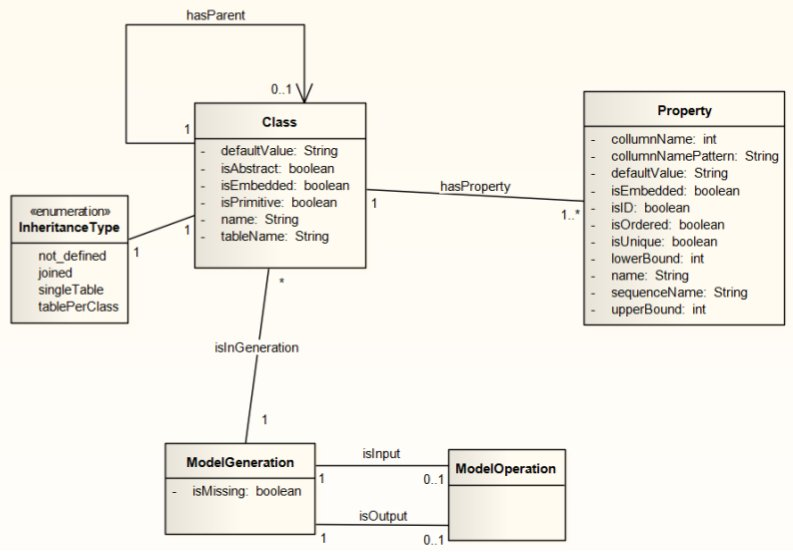
\includegraphics[width=15cm]{figures/app_meta_BP}
\caption{Aplikační metamodel v počátku vývoje obrázek převzat z \cite{Lukes}}
\label{fig:lukes:app_meta}
\end{center}
\end{figure}

\begin{figure}[ht]
\begin{center}
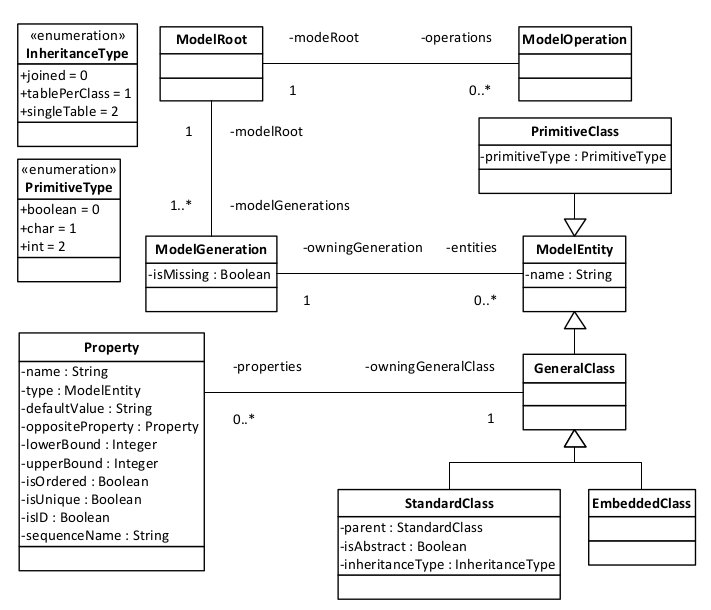
\includegraphics[width=15cm]{figures/app_meta_BP_jezek}
\caption{Aplikační metamodel v průběhu vývoje obrázek převzat z \cite{Jezek}}
\label{fig:jezek:app_meta}
\end{center}
\end{figure}

\begin{figure}[ht]
\begin{center}
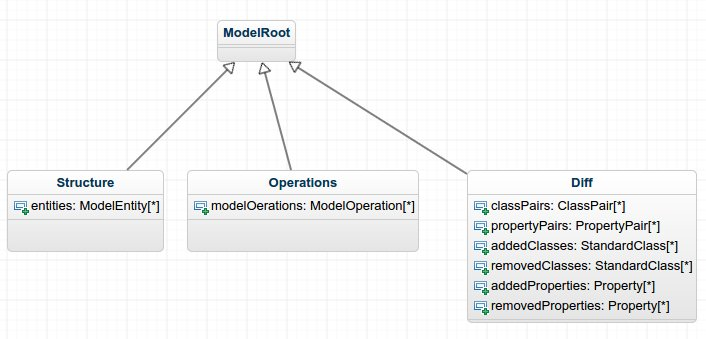
\includegraphics[width=15cm]{figures/app_roots}
\caption{Rootové elementy aplikačního modelu}
\label{fig:app_roots}
\end{center}
\end{figure}


\begin{figure}[ht]
\begin{center}
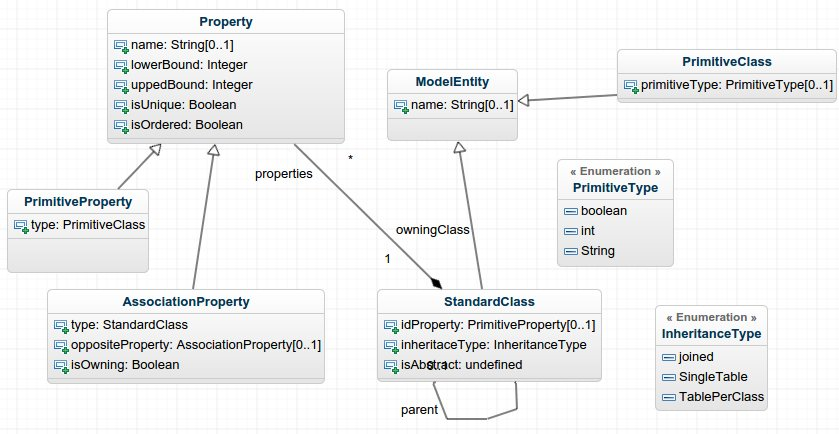
\includegraphics[width=15cm]{figures/app_meta}
\caption{Struktura aplikačního metamodelu}
\label{fig:app_meta}
\end{center}
\end{figure}

\section{Databázový metamodel}

Stejně jako aplikační model byl i model databázové struktury často upravován a v
konečném důsledku zjednodušován. Na obr. \ref{fig:rdb_str} vidíme aktuální
matamodel databázové struktury, na obr. \ref{fig:rdb_str_lukes} vidíme model na
počátku vývoje převzatý z \cite{Lukes} a na obrázku \ref{fig:rdb_str_tarant}
model v pozdější fázi vývoje převzatý z \cite{Tarant_bp}.

 Nejvýraznější změnami databázového modelu jsou - stejně jako v
 aplikačním metamodelu odstraněním generace modelů, odstranění elementu
 UnderlyingIndex, odstranění elementu ColumnConstraint, nahrazení elementu
 NotNullConstraint atributem boolean v Column a snížení kardinality Sequence
 obsažených ve schematu z * na 1.
 
 Myšlenka generace modelů byla zachována, ale jejich připadné uchovávání bylo
 zvoleno ve více oddělených souborech. Element UnderlyingIndex byl shládán
 nadbytečným, stejně jako element ColumnConstraint. Bezatributový element
 NotNullConstraint byl shledán příliš informačně chudým a byl nahrazen atributem
 isNillable zachovávajícím stejnou informační hodnotu jako element v původních
 modelech. 
	
\begin{figure}[ht]
\begin{center}
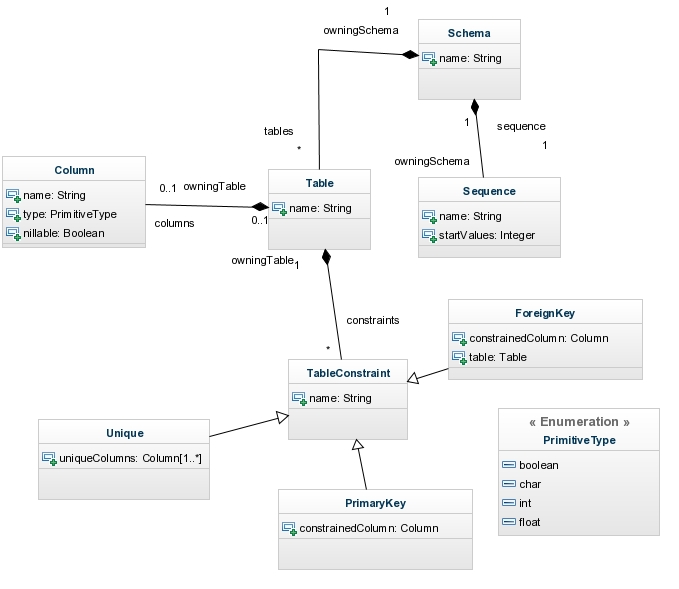
\includegraphics[width=15cm]{figures/rdb_structure}
\caption{Struktura databázového metamodelu}
\label{fig:rdb_str}
\end{center}
\end{figure}

\begin{figure}[ht]
\begin{center}
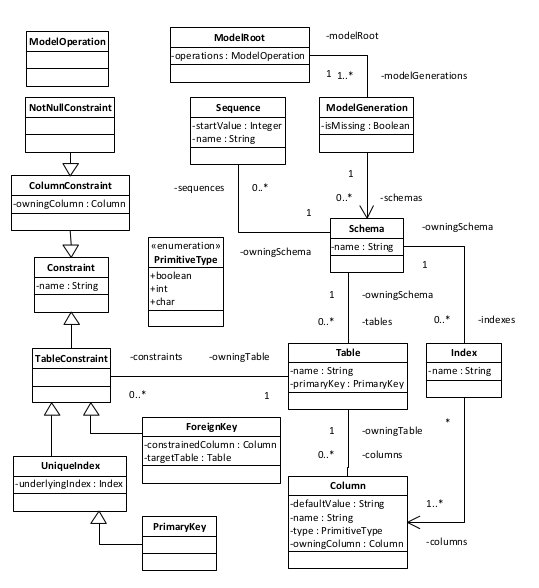
\includegraphics[width=15cm]{figures/rdb_structure_tarant}
\caption{Struktura databázového metamodelu v průběhu vývoje, obrázek převzat z
\cite{Tarant_bp}}
\label{fig:rdb_str_tarant}
\end{center}
\end{figure}

\begin{figure}[ht]
\begin{center}
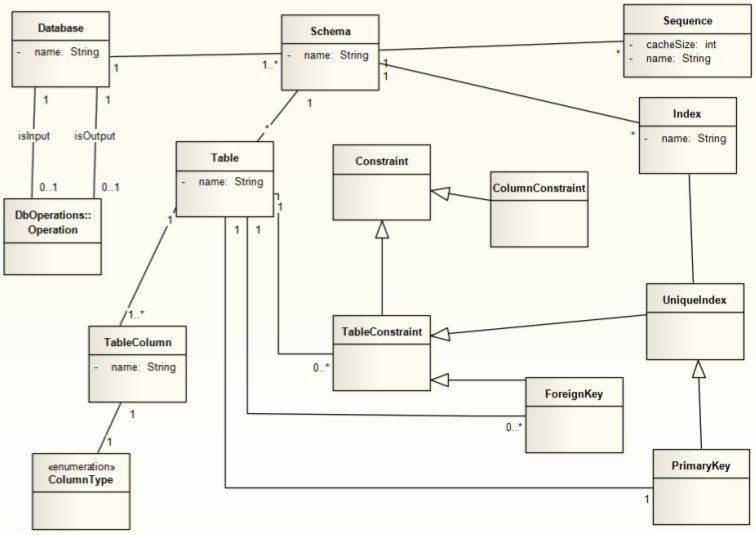
\includegraphics[width=15cm]{figures/rdb_structure_lukes}
\caption{Struktura databázového metamodelu v průběhu vývoje, obrázek převzat z
\cite{Lukes}}
\label{fig:rdb_str_lukes}
\end{center}
\end{figure}


\subsection{Operace nad aplikačním modelem}
\subsubsection{Cíle při modelování operací}

V průběhu modelování operací nad aplikačním modelem jsme se snažili, aby tyto
operace byly jednoznačné(strojově zpracovatelné) v rámci daného kontextu, dále
vzhledem k nutnosti textového zápisu uživatelem o minimalističnost zápisu. Tyto
dva koncepty jdou obecně proti sobě, proto jsme došli k jistému jejich
kompromisu uživatelské jednoduchosti zápisu a jednoznačnosti.

\subsubsection{Historický vývoj}

Operace v aplikačním modelu se vyvíjely a měnily se jejich parametry, ale
současně se měnil i seznam dostupných operací nad aplikačním modelem. Z operací
v první verzi modelu byly odstraněny operace MoveProperty, AddPrimitiveClass,
SetOpposite a SetType. Operace AddPrimitive byla označena za nadbytečnou,
protože není cílem modifikace modelu změna seznamu primitivních tříd, který
bývá definován použitým programovacím jazykem a tudíž by měl tento seznam být v
vstupní generaci.V průběhu analýzy operace SetOpposite bylo zjištěno, že tato
operace má smysl na strukturální úrovni, ale není možné ji aplikovat na obecná
data, proto byla tato operace nahrazena dvojicí operací ChangeUniToBidir a
ChangeBiToUnidir, které plní nároky kladené na původní operaci a jsou
aplikovatelné  na datové úrovni. Operace SetType byla prozkoumána, ale nebyla
exaktně popsána, nebylo nalezeno její mapování na operace v databázi ani
validační podmínky nutné k úspěšné aplikaci operace na aplikační model. Je
očekatelné, že by tato operace měla souviset s dědičnými hierarchiemi. 

\subsubsection{Seznam aplikačních operací}

Operace jsou uvedeny v tabulkách následujícím seznamu. Kromě
regulérních operací, které může vytvořit uživatel jsou v tabulce
zde uvedeny i virtuální operace DistributeProperty, MergeProperty a operace
ExportProperty, které jsou používány jako pomocné v implementaci složitějších
reduktivních a expanzivních operací a manipulují s Property v rámci dědičné
struktury tříd. Tyto operace mohou narozdíl od nevirtuálních operací být
aplikovány na model, který je z nějakého hlediska nevalidní. Například operace
MergeProperty počítá s hierarchií s kolizní property v třídě předka a
potomka. 

\newcounter{ListCitac}
\begin{list}{Operace \Roman{ListCitac}:}{\usecounter{ListCitac}}
  \item AddStandardClass(name, isAbstract, inHeritanceType)
  \begin{itemize}
    \item Validační podmínky - neexistuje třída s jménem nově vznikající
    \item Operace vytvoří novou třídu a její id odvozené z názvu třídy
  \end{itemize}
  \item RenameEntity(name, newName)
  \begin{itemize}
    \item Validační podmínky - existuje třída s původním jménem, neexistuje
    třída s novým jménem
    \item Operace změní název třídy na nový
  \end{itemize}
  \item SetAbstract(name, isAbstract)
  \begin{itemize}
    \item Validační podmínky - existuje třída s daným jménem
    \item Operace nastaví třídě atribut abstract na danou hodnotu    
  \end{itemize}
  \item RemoveEntity(name)
  \begin{itemize}
    \item Validační podmínky - existuje třída s daným jménem, neexistuje link na
    tuto třídu, třída neobsahuje žádné property, neexistuje pro tuto třídu žádný potomek
    \item Operace odstraní entitu (standardní třídu) z modelu
  \end{itemize}
  \item AddProperty(owningClassName, name, typeName, lowerBound, upperBound,
  isOrdered, isUnique) 
  \begin{itemize}
    \item Validační podmínky - zadané bounds jsou validní, v hierarchii
    dědičnosti neexistuje kolizní property se stejným jménem
    \item  Operace vytvoří v dané třídě novou property se zadanou horní mezí,
    dolní mezí, typem, seřaditelností a unikátností
  \end{itemize}
  \item RenameProperty(owningClassName, name, newName)
  \begin{itemize}
    \item Validační podmínky - existuje přejmenovaná property v dané třídě,
    nexistuje property v dané třídy nového jména
    \item  Operace změní název property v dané třídě ze starého na nový
  \end{itemize}
  \item RemoveProperty(owningClassName, name)
  \begin{itemize}
    \item Validační podmínky - musí exitovat vlastnická třída property a v ní
    odstraňovaná property
    \item  Operace odstraní property z dané třídy
  \end{itemize}
  \item SetBounds(upperBound, lowerBound)
  \begin{itemize}
    \item Validační podmínky - bounds musí být validní a musí existovat daná
    trída a property
    \item  Operace nastaví horní a dolní mez property na nové hodnoty
  \end{itemize}
  \item SetOrdered(owningClassName, name, isOrdered)
  \begin{itemize}
    \item Validační podmínky - musí existovat daná trída a property
    \item  Operace nastaví property seřaditelnost
  \end{itemize}
  \item SetUnique(owningClassName, name, isUnique)
  \begin{itemize}
    \item Validační podmínky - musí existovat daná třída a property
    \item  Operace nastaví property unikátnost
  \end{itemize}
  \item AddParent(className, parentClassName)
  \begin{itemize}
    \item Validační podmínky - musí existovat rodičovská třída a třída potomka,
    třída potomka nesmí mít nastaveného rodiče
    \item Operace nastaví třídě předka a přesune překrývající atributy do
    rodičovské třídy
  \end{itemize}
  \item RemoveParent(className, parentClassName)
  \begin{itemize}
    \item Validační podmínky - musí existovat třída child a mít nastavenou
    rodičovskou třídu
    \item Operace odstraní třídě rodičovskou třídu a rozdistribuje (použije
    virtuální operaci distribute property) property z rodičovské třídy do třídy původního potomka
  \end{itemize}
  \item ExtractClass(sourceClassName, extractClassName, associationPropertyName, oppositePropertyName, propertyNames)
  \begin{itemize}
    \item Validační podmínky - musí existovat zdrojová třída, neexistuje
    property s jménem linku na nově vzniklou třídu, existují exportované property
    \item Operace vytvoří novou třídu, kterou napojí na původní třídu,
    exportuje(využije virtuální operaci export property) do nově vzniklé třídy
    vyjmenované property
  \end{itemize}
  \item InlineClass(targetClassName, associationPropertyName)
  \begin{itemize}
    \item Validační podmínky - musí existovat cílová třída a
    musí existovat asociační property typu Inlinované třídy, která má upper
    bound 1
    \item Operace exportuje všechny property z inlinované třídy do cílové třídy
    přes specifikovanou unidirectional asociaci
  \end{itemize}
  \item ChangeUniToBidir(className, associationPropertyName, oppositePropertyName)
  \begin{itemize}
    \item Validační podmínky - v dané třídě musí existovat asociační property
    s daným jménem a nesmí mít nastavenou opposite property 
    \item Operace vytvoří nový zpětný link s oppositePropertyName k property
    targetClassName a nastaví správně data do opepositePropertyName
  \end{itemize}
  \item ChangeBiToUnidir(className, associationPropertyName)
  \begin{itemize}
    \item Validační podmínky - v dané třídě musí existovat asociační property
    s daným jménem a musí mít nastavenou opposite property
    \item Operace odstraní opoziční property
  \end{itemize}
  \item CollapseHierarchy(superClassName, subClassName, isIntoSub)
  \begin{itemize}
    \item Validační podmínky - musí existovat subclass a superclass, subclass
    musí mít nastavenou superclass jako parenta
    \item Operace exportuje (aplikuje virtuální operaci) všechny property z
    jedné třídy do jejího předka a třídy spojí, upraví dědičné vazby
  \end{itemize}
  \item ExtractSubClass(sourceClassName, extractedClassName, extractedPropertyNames)
  \begin{itemize}
    \item Validační podmínky - musí existovat třída s name sourceClassName a
    nesmí existovat třída s jménem extractedClassName, v třídě sourceClass musí
    existovat property s názvy z kolekce extractedPropertyNames
    \item Operace vytvoří třídě nového potomka a
    exportuje(aplikuje virtuální operaci export property) do něj vyjmenované property
  \end{itemize}
  \item ExtractSuperClass(sourceClassesName, extractParentName, propertyNames)
  \begin{itemize}
    \item Validační podmínky - musí existovat třída s name sourceClassName a
    nesmí existovat třída s jménem extractedParentName, v třídě sourceClass musí
    existovat property s názvy z kolekce propertyNames
    \item Operace vytvoří třídě nového předka a přesune do něj vyjmenované
    property, pokud měla původní třída předka nastaví tohoto předka rodičem 
    nově vzniklé třídě
  \end{itemize}
  \item PullUpProperties(childClassName, pulledPropertiesNames)
  \begin{itemize}
    \item Validační podmínky - musí existovat childClass a mít nastavenou
    rodičovskou třídu, v třídě potomka musí existovat properties z kolekce
    pulledPropertiesNames, v okolních subhierarchiích nesmí existovat properties
    z této kolekce
    \item Operace exportuje(aplikuje virtuální operaci export property) property
    do rodičovské třídy
  \end{itemize}
  \item PushDownProperties(childClassName, pushedPropertiesNames)
  \begin{itemize}
    \item Validační podmínky - musí existovat class s childClassName a mít
    nastavenu parentClass, v třídě potomka musí existovat properties z kolekce
    pushedPropertiesNames
    \item Operace exportuje(aplikuje virtuální operaci export property) 
   vyjmenované property do třídy potomka a přesune JEN data potomka
  \end{itemize}
  \item ExportProperty(exportedPropertyName, className)
  \begin{itemize}
    \item virtuální operace
    \item Operace přesune property a data v ní obsažená v rámci hierarchie do
    cílové třídy
  \end{itemize}
  \item DistributeProperty(distributedPropertyName, className)
  \begin{itemize}
    \item virtuální operace
    \item Operace zduplikuje strukturu v rámci hierarchie dané property do
    cílové třídy a přesune data přiřazená této třídě
  \end{itemize}
  \item MergeProperty(mergedPropertyName, className)
  \begin{itemize}
    \item virtuální operace
    \item Operace přesune data zdrojové property do cílové property a smaže
    strukturu původní property
  \end{itemize}
\end{list}

\subsubsection {Rozdělení aplikačních operací} 

Operace nad aplikačním modelem je možné dělit podle dvou kritérií - 1. nad jakým
typem entity pracují, 2. jaký je charakter/význam pro tito entity daná operace
má.

První kritérium dělí aplikační operace na operace pracující s třídami a operace
pracující pouze s properties daných tříd. Příkladem operací pracujících s
třídami jsou operace AddStandardClass, AddParent a RemoveEntity. Příkladem
operací pracujících s properties jsou operace AddProperty, RemoveProperty,
SetAbstract.

Podle druhého kritéria je možné rozdělit operace nad aplikačním modelem 5 skupin
- konstruktivní, destruktivní, expanzivní, reduktivní a modifikační operace.
Konstruktivní operace jsou takové, které po své aplikaci vytvoří 1 novou entitu
v výsledném modelu, která nemá žádné vazby na jiné entity. Příklady aditivní
operace je operace AddClass. 

Destruktivní operace je opak konstruktivní, v vstupním modelu existuje entita a
ta je aplikaci destruktivní operace odstraněna. Příkladem destruktivní operace
je operace RemoveProperty.

Operace expanzivní přídává do výstupního modelu jednu entitu, čímž se
podobá operaci konstruktivní, nicméně zároveň je vázána na jinou entitu stejného typu a
zmenšuje její obsah. Příkladem expanzivní operace je ExtractClass. 

Reduktivní operace entitu z vstupního modelu odstraní a zároveň entitě, která
je pro operaci řídící změní obsah. Příkladem této operace je InlineClass.
Reduktivní operace jsou inverzní k operacím expanzivním.\\

Rozdělení operací nad aplikačním modelem je jen formální, neprojevilo se změnou
hierarchické struktury operací. Struktura operací byla zjednodušena - již
neexistuje rozhlodatelná operace ComposedOperation, všechny operace jsou nyní
defakto atomické. Tato změna byla zapříčiněna neschopností rozložit některé
dekomponovatelné operace na operace atomické. Je zde nutné podotknout, že tento
rozklad je v nynější chvíli možný, ačkoliv si vyžádal neformální
obohacení aplikačního modelu o některé atomické operace jakými jsou
mergePropery, distributeProperty a exportProperty. Tyto operace v aplikačním
modelu neexistují, ale v rámci transformace ORMo jsou v metodách
použity/volány.\\


\subsection{Delta notace}
V \cite{Cincetti} jsou definovány operace pomocí delta notace. Delta notace
je taková, která ukazuje všechny změny mezi danými dvěma artefakty stejné
úrovně abstrakce. Změnami můžeme rozumět přidáním elementu, odstraněním elementu
a modifikací elementu.


Nejznámějším a nejrozšířenějším typem delta notace je výstup linuxového
příkazu diff. Každý rozdíl v delta notaci příkazu diff je dle
\cite{diff_wiki} definován následně:

\begin{verbatim}
popis změny
<řádek z prvního souboru
<řádek z prvního souboru…
---
>řádek ze druhého souboru
>řádek ze druhého souboru…
\end{verbatim}

Popis změny může nabývat tvaru: LaR, FcT nebo RdL.\\

\begin{itemize}
   	\item [LaR ] \hfill \\
   		Ve druhém souboru jsou navíc řádky R patřící za řádek L prvního souboru. 
    	Např. 8a12, 15 znamená, že ve druhém souboru jsou navíc řádky 12-15 a patří
    	za řádek 8 v prvním souboru.
	\item [FcT] \hfill \\
		Řádky F z prvního souboru byly změněny. Ve druhém souboru jsou jim
		odpovídající řádky T. Např. popis 5,7c8,10 znamená, že se liší řádky 5-7 v
		prvním souboru a jim odpovídající jsou řádky 8-10 ve druhém souboru.	 
  \item [RdL] \hfill \\
		Ve druhém souboru chybí řádky R z prvního souboru. Tyto řádky by patřily za
		řádek L druhého souboru. Např. 5,7d3 znamená, že za řádkem 3 ve druhém souboru
		chybějí řádky 5-7 prvního souboru.	  
\end{itemize}


Příklad Delta notace za pomoci linuxových
nástrojů diff dvou souborů\\
\begin{lstlisting}[language=JAVA,frame=single,caption=Man1.java,label=Man1]
class Man {
	private String name;

	public Man(String name){
		this.name = name;
	}

}
\end{lstlisting}

\begin{lstlisting}[language=JAVA,frame=single,caption=Man2.java,label=Man2]
class Man {
	private String name;

	private String surename;

	public Man(String name){
		this.name = name;
	}

	public Man(String name, String surename){
		this(name);
		this.surename = surename;
	}
}
\end{lstlisting}

\begin{lstlisting}[language=JAVA,frame=single,caption=Diff Man1
Man2,label=Diff_1_2]
3a4,5
> 	private String surename;
> 
5a8,12
> 	}
> 
> 	public Man(String name, String surename){
> 		this(name);
> 		this.surename = surename;	
\end{lstlisting}

Ukázka kódu \ref{Man1} zobrazuje zdrojový kód třídy Man v první
verzi. Ukázka \ref{Man2} potom zdrojový kód třídy Man po první naší editaci,
kdy jsme do dané třídy přidali nový atribut a nový konstruktor.
Diff v delta notaci těchto dvou souborů je ukázán v \ref{Diff_1_2}. V delta
notaci vidíme, že do prvního souboru byly za 3. řádek vloženy řádky 4-5 z
druhého souboru - řádek definující nový atribut surename a oddělující prázdný
řádek, dále za 5. řádek byly vloženy řádky 8-12 z druhého souboru definující
nový konstruktor a uzavírací závorka.\\

Delta notace je dle autora výhodná díky snadné
rozložitelnosti velkých patchů na více menších patchů a také díky oddělení ve
více konkurenčních patchích konfliktních operací od operací nazávislých. 

Inverzní diff vidíme v \ref{Diff_reverse}, kde z souboru
\ref{Man2} byly odstraněny řádky 4-5, které by se jinak zařadily za řádek 3,
dále byly odstraněny řádky 10-13, které by jinak patřily za řádek 7 souboru
Man1.


\begin{lstlisting}[language=JAVA,frame=single,caption=patch
$part_b$,label=Diff_reverse]
4,5d3
< 	private String surename;
< 
8,12d5
< 	}
< 
< 	public Man(String name, String surename){
< 		this(name);
< 		this.surename = surename;
\end{lstlisting}

Patch \ref{Diff_1_2} bychom mohli rozdělit například na \ref{Diff_1_2_a} a
\ref{Diff_1_2_b}, protože změny jsou na různých řádcích a jsou zdánlivě
nezávislé. Aplikací těchto dvou patchů v pořadí $part_a$ a $part_b$ vznikne
\ref{Man1_alternative}, kdežto aplikace patchů v pořadí $part_b$, $part_a$ dá
vzniknout původnímu souboru \ref{Man2}

\begin{lstlisting}[language=JAVA,frame=single,caption=patch
$part_a$,label=Diff_1_2_a]
3a4,5
> 	private String surename;
> 
\end{lstlisting}

\begin{lstlisting}[language=JAVA,frame=single,caption=patch
$part_b$,label=Diff_1_2_b]
5a8,12
> 	}
> 
> 	public Man(String name, String surename){
> 		this(name);
> 		this.surename = surename;	
\end{lstlisting}

\begin{lstlisting}[language=JAVA,frame=single,caption=aplikace pořadí
difů $part_a part_b$,label=Man1_alternative] 
class Man {
	private String name;

	private String surename;

	}

	public Man(String name, String surename){
		this(name);
		this.surename = surename;
	public Man(String name){
		this.name = name;
	}

}\end{lstlisting}


Delta notace umožňuje snadný forward i backward differencing, protože díky
kontextové nezávislosti je možné snadno invertovat operace. Kontextová nezávislost znamená,
že jakýkoliv patch je možné aplikovat na jakýkoliv model, přičemž očekávatelný
výsledek je výstupní soubor nebo chyba. Přidávání řádků do souboru je vždy
aplikovatelné. Náhrada a odstranění řádků ze souboru, ve kterém nefigurují
naopak vyvolá chybu. 

Aplikace patche \ref{Diff_1_2} na \ref{Man2} by vypadala \ref{Man2_p1_2}.
Atribut byl přidán na správné místo, ale konstruktor byl přidán na místo špatné 
- přídaná uzavírací závorka neuzavírá předchozí konstruktor, ale celou třídu. 
Navzdory tomu, že tento Java kód je nevalidní, patch bylo možné aplikovat.\\

\begin{lstlisting}[language=JAVA,frame=single,caption=patch
aplikován na třídu Man2,label=Man2_p1_2]
class Man {
	private String name;

	private String surename;

	private String surename;

	}

	public Man(String name, String surename){
		this(name);
		this.surename = surename;
	public Man(String name){
		this.name = name;
	}

	public Man(String name, String surename){
		this(name);
		this.surename = surename;
	}
}
\end{lstlisting}

Všimněme si, že standardní unixový diff obsahuje redundantní informaci -
řádek \ref{Diff_1_2_a} 3a4,5 musí obsahovat číslo řádku, za který se má
navazující text diffu přidat, ale nemusí obsahovat, na které pozice v
druhém souboru budou přidány, tato informace by byla dopočitatelná z aplikace
všech předchozích řádků, přičtení počtu řádků přidávaných a odečtení řádků
odebíraných. Takovouto změnou standardní delta notace dostaneme další možnou
variantu delta notace.

Standardní delta notace obsahuje další redundantní prvky. Například v deltě
mazající řádky je redundantní informací seznam mazaných řádků. Jeho odstraněním
bychom získali plně operaci aplikovatelnou na jakýkoliv model. Tato změna
nevytváří delta notaci - neuchovává všechny informace o změně modifikovaných
elementů. Pro ilustraci diff na \ref{reverse_add_1_2} je reverzní vůči diffu
\ref{Diff_1_2}. Odstraněním seznamu mazaných řádků a pozice v druhém souboru
získáme diff \ref{delete_minimal}. Z tohoto vyplývá, že delta notace není
minimální, obsahuje redundatní informace. Prostým pozorováním můžeme zjistit,
že oproti delta notaci nemůže v nově vzniklé minimální notaci být odvozena
inverze \ref{Diff_1_2} diffu \ref{delete_minimal}, obrácený postup -
transformace diffu \ref{Diff_1_2} na \ref{delete_minimal} bez znalosti
kontextových modelů \ref{Man1} a \ref{Man2} je naopak zachována z delta notace.
Nově vzniklá notace je tudíž neidempotentní vůči operaci inverze bez znalosti
kontextového vstupního a výstupního modelu. 

\begin{lstlisting}[language=JAVA,frame=single,caption=diff
modelů 2 a 1,label=reverse_add_1_2] 
4,5d3
< 	private String surename;
< 
10,13d7
< 	public Man(String name, String surename){
< 		this(name);
< 		this.surename = surename;
< 	}
\end{lstlisting}

\begin{lstlisting}[language=JAVA,frame=single,caption=diff
modelů 2 a 1,label=delete_minimal] 
4,5d
10,13d7
\end{lstlisting}

\subsubsection{Vlastnosti operací}
V \cite{Cincetti} jsou popsány některé specifické vlastnosti jako
je invertovatelnost a rozložitelnost operací. Je nutné říci, že operace
zmiňované v literatuře pracují jen se strukturou dat, nikoliv s daty samotnými a jsou
kontextově nezávislé - tyto operace jsou tvořeny téměř výlučně konstruktivními
a  destruktivními operacemi. (intensional vs extensional - první potřebuje
konkrétní model ke své aplikaci, druhá ne, extensional je možné použít na
paralelní vývojové větve).

V projektu Migdb na druhé straně existují operace,
které jsou kontextově závislé, což je uživatelskou přívětivostí  operací - jako
zástupcem takové operace se dá uvést operace AddParent(parentClass=B,
childClass=A), která nezmiňuje všechny Property,  které se mají odstranit, ale
dynamicky si je dopočítává v závislosti na daném kontextu. Její inverzí je
operace RemoveParent(childClass=A). Vzhledem k minimalističnosti neexistuje k
operaci RemoveParent(childClass=A) jednoznačná inverze bez daného konktextu.

Inverzi AddParent(sourceClass=A parentClass=B) získáme, pokud v
kontextu přidruženém modelu aplikaci RemoveParent má třída A předka B. Nicméně i
v takovém případě neplatí, že aplikace sekvence těchto dvou inverzních operací
na vstupní model M vygeneruje vždy původní model. Příkladem tohoto neočekávaného
chování je vstupní model Man(int age, String name), Person(int age, String name, String sureName).
Aplikace operace AddParent(Man, Person) odstraní přebytečné atributy v třídě man
a přidá rodiče této třídě, tj vznikne model : Man()->Person, Person(int age,
String name, String sureName). Nyní je aplikována operace RemoveParent(Person),
která sice získá z modelu jméno rodičovské třídy, ale nezíská seznam property,
které se distribuují do třídy Man. Operace byly navrženy tak, aby maximalizovali
objem zachovaných dat, proto operace RemoveParent distribuuje všechny
atributy třídy Person do třídy Man. Výsledný model je tedy: Man(int age, String
name, String sureName), Person(int age, String name, String sureName) a odlišuje
se od vstupního modelu o property sureName v třídě Man.

Stejná vlastnost platí pro dvojici ChangeUniToBidir a ChangeBiToUnidir, s
rozdílem, že se nejedná o automaticky získanou rodičovskou třídu, ale
opozitní property.

\section{Databázové operace}



\section{ORMo (ORM operací)}

Ačkoliv v průběhu projektu Migdb byla transformace operace z aplikačního modelu
na sadu operací databázových označována jako ORM operací, zkráceně ORMo,
Ačkoliv na úrovni aplikační všechny operace fungují se všemi inheritanceTypy 
bylo nutné zjednodušit aplikační model tak, aby byla transformace ORMo
implementovatelná, proto jsme v rámci týmu Migdb rozhodli o redukci počtu
inheritanceTypů na jeden - nejvhodnější typ je nejspíše joined, který je
pravděpodobně nejpoužívanějším.
Vzhledem k nedostatku času nebyla implementována myšlenka .q souborů, které
kontrolují některé vlastnosti nejen modelu, ale i konkrétních dat, dále není
mapováno omezení LB = 0, které by některé operace stížilo. Algoritmus ORMo si
bere všechna data z aplikačního modelu, čímž je nezávislý na aplikaci
databázových operací nad databázovým modelem, ale předává veškerou zodpovědnost
za údržbu - tj vytvoření a odstranění omezení.
V tabulkách \ref{tab:odbchmSeznam1} a \ref{tab:odbchmSeznam1} nejsou uvedena
vytváření a odstraňování unikátních constrainů pro unikátní či ordered kolekce
primitivních a neprimitivních typů.

V tabulkách 

\begin{table}
\begin{center}
\begin{tabular}{| c|| p {6cm}|}
\hline
\bfseries Název operace &
\bfseries Rozklad na db operace \\[2mm] 
\hline \hline
AddStandardClass &   Vytvoří tabulku, id sloupec této tabulky a primární klíč\\
\hline
RenameEntity & Operace změní název tabulky na nový, odstraní a vytvoří PK s
novým jménem\\
\hline
SetAbstract & pro isAbstract = true maže data, která náleží pouze dané třídě\\
\hline
RemoveEntity & V Db je smazán primární klíč, id property a tabulka
odpovídající dané třídě\\
\hline
AddProperty & operace přidá do cílové tabulky sloupec pro primitivní property S UB = 1\\
\ & operace přidá tabulku, datový sloupec, referenční sloupec a referenci na vlastnickou tabulku pro primitivní 
property s UB = > 1\\
\ & operace přidá sloupec pro neprimitivní property S UB = 1 do vlastnické tabulky a referenci na tabulku typu\\
\ & operace vytvoří vazební tabulku pro neprimitivní property s UB > 1, vloží do ní referenční sloupce na 
vlastnickou tabulku a tabulku typu, na které vytvoří cizí klíč\\
\hline
RenameProperty & pro danou 
property s UB = 1 a primitivním typem přejmenuje property v vlastnické tabulce\\
\ & pro danou primitivní property s UB > 1 přejmenuje datový sloupec, FK na vlastníka kolekce a tabulku kolekce \\
\ & pro danou associační property přejmenuje sloupec v vlastnické tabulce a cizí klíč referující tabulku typu\\
\ & pro danou asociační property přejmenuje vazební tabulku s referenčními sloupci na vlastníka a typ asociace + 
cizí klíče \\
\hline
RemoveProperty & pro primitivní property S UB = 1 odstraní sloupec z dané
tabulky\\
\ & pro danou property primitivního typu s UB > 1 odstraní referenci na vlastnickou tabulku, sloupec z tabulky 
dané kolekce, datový sloupec a smaže kolekční tabulku \\
\ & pro danou asociační property s UB = 1 odstraní referenci na tabulku vlastníka a referenční sloupec\\
\ & pro danou asociační property s UB > 1 odstraní reference na vlastnickou tabulku a tabulku typu, datový 
sloupec a sloupec typu a smaže vazební tabulku \\
\hline
SetBounds & NEIMPLEMENTOVÁNO \\
\hline
SetOrdered & pro nastavní = true přidá sloupec ordering, (měl by přenastavit 
data) a vytvoří unikátní constraint přes typový, referenční a orgering sloupec\\
\ & pro nastavení = false smaže ordering constraint a ordering column\\
\hline
SetUnique & owningClassName, name, isUnique \\
\hline
AddParent &  Aplikuje obraz operace MergeProperty na všechny kolizní property,
přidá cizí klíč na rodičovskou třídu\\
\hline
RemoveParent & aplikuje obraz operace DistrubuteProperty na všechny property
rodičovské třídy, odstraní cizí klíč, smaže data třídy potomka z tabulky rodiče\\
\hline
ExtractClass & vytvoří novou tabulku, aplikuje obraz operací exportProperty pro 
každou exportovanou property\\
\hline 
InlineClass & aplikuje obraz operací exportProperty, smaže linkProperty a
Inlinovanou tabulku\\
\hline
ChangeUniToBidir & pro associační property vytvoří sloupec a nastaví validně opposite  \\
\hline
ChangeBiToUnidir & className, associationPropertyName \\
\hline
\end{tabular}
\end{center}
\caption{ODBCHM Seznam operací část 1}
\label{tab:odbchmSeznam1}
\end{table}

\begin{table}
\begin{center}
\begin{tabular}{| c|| p{5cm}|p {6cm}|}
\hline
\bfseries Název operace & \bfseries popis &
\bfseries parametry \\[2mm] 
\hline \hline
CollapseHierarchy & Exportuje property z jedné třídy do jejího předka a třídy
spojí, upraví dědičné vazby & superClassName, subClassName, isIntoSub\\
\hline
ExtractSubClass & Vytvoří třídě nového potomka a přesune do něj vyjmenované
property & sourceClassName, extractedClassName, extractedPropertyNames\\
\hline
ExtractSuperClass & Vytvoří třídě nového předka a přesune do něj vyjmenované
property, pokud měla původní třída předka nastaví tohoto předka rodičem nově
vzniklé třídě & sourceClassesName, extractParentName, propertyNames \\
\hline
PullUpProperties & Exportuje property do rodičovské třídy & childClassName,
pulledPropertiesNames\\
\hline
PushDownProperties & Exportuje vyjmenované property do třídy potomka a přesune JEN data potomka &
childClassName, pushedPropertiesNames\\
\hline
ExportProperty(virtuální operace) & Exportuje property v rámci hierarchie a data do cílové třídy & exportedPropertyName, 
className\\
\hline
DistributeProperty(virtuální operace) & Zduplikuje strukturu dané property do cílové třídy a přesune data přiřazená 
této třídě & DistributedPropertyName, className\\
\hline
MergeProperty(virtuální operace) & Přesune data zdrojové property do cílové property a smaže strukturu původní property & 
mergedPropertyName, className\\
\hline
\end{tabular}
\end{center}
\caption{ODBCHM Seznam operací část 2}
\label{tab:odbchmSeznam2}
\end{table}

\subsection{Diff elementy}

 Kvůli nutnosti rozpoznávat operace vznikly v aplikačním modelu nové
 elementy. Kořenovým elementem diff modelu je Diff element. Tento element
 obsahuje kolekce elementů classpairs typů ClassPair, propertyPairs
 typu PropertyPair, a dále pak addedClasses a removedClasses typu DiffClass a
 addedProperties a removedProperties typu DiffProperty. Element ClassPair
 shlukuje zpárované zdrojové (source) a obrazové (reflection) třídy, dále pak
 referenci owningDiff na Diff element, v kterém jsou obsaženy a která je
 důležitá pro implementaci algoritmu a v neposlední řadě underlyingPairs -
 shodné páry Properties typu EqualPropertyPair, které jsou detekované danou
 operací. Podobně jako operace jsou i páry rozděleny do několika rodin.
 Konstruktivní a destruktivní operace nemají svůj obraz v diff metamodelu - tyto
 operace nemapují vzniklý nebo odstraněný element na jakýkoliv jiný element.
 
 Oproti jednodušším konstruktivním a destruktivním operacím jsou operace
 expanzívní, konstruktivní a modifikační v Diff modelu zobrazeny jako
 ExpansiveClassPair, ReductiveClassPair a ModifyingClassPair, mapují element
 vstupního modelu na element cílového modelu. Aby bylo možné rozpoznat
 specifický pár závislý na jiném páru, byla přidána třída ReplacingClassPair -
 nahrazující pár, který se používá jako pivot pro hledání expansivních, 
 reduktivních a modifikačních párů. Od elementu ReplacingClassPair dědí elementy
 EqualClassPair - třída, která si uchovala jméno z původního modelu a element
 ReplacingClassPair - reprezentující třídu, která si neuchovala jméno, ale má
 změněný název. Podmínky získávání konkrétních typů párů a jejich pořadí
specifikuje konkrétní rozpoznávací algoritmus.
 
 Projevem subtraktivních a aditivních operací jsou elementy DiffClass a
 DiffProperty, které zaobalují třídy a property tak, aby bylo možné referencovat
 na jiný objekt než element Structure. 

\section{Rozpoznávání operací}

Algoritmem pro rozpoznávání operací nazveme každý algoritmus, který nám pro
každý vstupní model A a cílový model B najde uspořádaný seznam operací, jejichž
postupná aplikace transformuje model A do modelu B. Tento algoritmus nemusí být
deterministický.

Jedním z zajímavých faktů je poznatek, že seznam operací nemusí být jednoznačný
a to i u jednoduchých změn. Pokud aplikujeme sekvenci operaci Inline A, B + 
Rename B ->C na model X dostaneme stejný výstup jako aplikací operací Inline B,
A + Rename A->C, ještě zajímavějším poznatkem je, že nejsme schopni rozeznat
rozdíl mezi aplikací sekvence operací Rename A, C + Inline C, B.

Samostatným tématem je pořadí operací a jeho permutace. Je zřejmé, že pořadí v
seznamu operací operujících nad jinými elementy bude možné libovolně prohazovat.
Také je samozřejmé, že seznam subtraktivních operací je také možné libovolně
zpermutovat. Stejně tak seznam aditivních operací. Obecný princip seřazení kolekce 
operací není znám. 

\section{Obecné principy model matching}
Jak je diskutováno v 19 a Different Models for Model Matching:
An analysis of approaches to support model differencing existuje několik
požadavků na algoritmus řešící problém model matching. Tyto požadavky zahrnují
přesnost, vysokou míru abstrakce na které je porovnávání provedeno, nezávislost
na konkrétních nástrojích, doménách a jazycích (přelož independence from
particular tools), použitelnost(efficiency) a minimální nutnost adaptace
algoritmus pro daný problém. Tyto požadavky jdou proti sobě a je nutné
preferovat některé na úkor jiných, proto není možné označit za nejlepší, ale je
nutné vybrat si správný algoritmus v závislosti na řešeném problému.

Nejtriviálnější implementovatelný algoritmus by mohl smazat zdrojový model
pomocí destruktivních operací a následně vytvořit výsledný model pomocí operací
konstruktivních, připadně poupravit atributy jednotlivých elementů pomocí
operací modifikačních. Argumentem proti použití takového algoritmu je smazání jakýchkoliv dat, které v
původní databázi byla a dobré si uvědomit, že funkci vytvoření DB modelu zvládá
ORM mapování integrované do většiny současných IDE.

 V literatuře (Different Models for Model Matching:
An analysis of approaches to support model differencing) byly popsány algoritmy
pro mapování shodných entit modelů (ModelMatching) a algoritmy pro získávání rozdílu modelů (Model Diff).
 Principem těchto modelů je párování elementů vstupního modelu s elementy z
 modelu cílového. Existují 4 obecné skupiny dělení matching algoritmů. 1
 párování podle statického identifikátoru, 2. signature based matching, 3.
 similarity based matching a custom language specific matching.
 
 Párování podle statického identifikátoru páruje elementy podle perzistentního
 identifikátoru, který je přiřazen každé entitě v době jejího vzniku, je
 neměnný a unikátní. Nejzákladnějším principem model matchingu je tedy párování
 entit na základě shodnosti jejich identifikátorů. Tento princip má výhody
 jednoduchosti implementace a rychlosti. Tento algoritmus není použitelný pro
 modely vytvořené nezávisle jeden na druhém či u technologií nepodporujících
 maintenance unikátních identifikátorů.
 
 Algoritmus signature based matching byl navržen kvůli limitaci párování podle
 statického identifikátoru, tento algoritmus je založen na dynamickém vypočtení
 nestatické signatury jednotlivých features pomocí uživatelem definovaných
 funkcí specifikovaných pomocí nějakého dotazovacího jazyka. Tento princip tedy
 může být použit pro modely vzniklé nezávisle na sobě. Nevýhodou je potom
 nutnost specifikovat query, které dopočítají signaturu.
 
 Algoritmus Similarity based matching používá podobně jako signature based
 matching podobnost features jednotlivých elementů, kterou agreguje do skalární hodnoty.
 Tento princip se řadí mezi podtyp attribute graph matchingu. Každá feature
 modelu může mít jinou váhu pro porovnávání, napřiklad u podobnosti tříd má
 jméno vyšší důležitost nežli abstractnost dané třídy.  Tento algoritmus musí
 být typicky doplněn o konfiguraci vah jednotlivých features elementů, kterou
 většinou píše vývojář. Zástupcem tohoto principu je framework EMF Compare, 
 který je doplněn o defaultní konfiguraci vah. Výhodami je větší přesnost,
 nevýhodou je potom TRIAL ERROR metoda získávání vhodné konfigurace vah.
 
 Algoritmy v kategorii Custom language specific matching jsou vytvořené
 přímo k využití daného modelovacího jazyka. Hlavní výhodou je, že
 algoritmus na dané doméně může začlenit do metody similarity based matchingu
 sémantické detaily, což vede k přesnějším výsledkům a redukuje prohledávaný 
stavový prostor. Jako příklad je uváděn jazyk UMLDiff, který při porovnávání
dvou UML modelů může využít faktu, že dvě třídy nebo dva datové typy
stejného jména tvoří po všech praktických stránkách pár(match). Nicméně výhoda
začlenění sémantických detailů konkrétní domény je vykoupeno vysokou cenou -
všechny ostatní kategorie algoritmů potřebují minimální neb téměř žádné úpravy
od vývojáře, pro tuto kategorii vývojáře musí napsat celý matchovací algoritmus
sám.

\subsection{Graph matching}
 Problém model matching je podproblémem generičtějšího tasku graph matching,
 který studuje http://www.sc.ehu.es/acwbecae/ikerkuntza/these/Ch2.pdf a
 rozděluje a popisuje algoritmy pro graph matching. Problém je definován na
 obecné struktuře Graf, což je uspořádaná dvojice G = (V, E), kde G je množina
 uzlů a E je množina hran grafu, přičemž $E \subset V \times V$. Grafy mohou být
 orientované či neorientované, mohou mít vícenásobné hrany.
 
 Každý graf může přidávat informace do své struktury pomocí labelu (popisku
 nebo číslu) do hran a vrcholů, pokud je nutné přidat více informací, je možné
 přidat do hran a/nebo vrcholů atributy, potom hovoříme o vertex-atributed
 grafech a edge atributed grafech, případně attributed grafech. V některé
 literatuře jsou attributed grafy označovány jako labeled grafy. Graph
 matching je aplikován v mnoho oborů jako je počítačové vidění, analýza
 scény(scene analysis), chemie a molekulární biologie. V těchto oborech musí být
 vzorce nalezeny v daných datech. 
  
 Problém graph matchingu dvou grafů $G_P$ (grafu patternu) a $G_M$ (grafu
 modelu), přičemž se dělí podle převzatého obrázku \ref{fig:graph_matching} na
 matching nalezení přesné shody vzorku v hledaném grafu či matching hledání
 podobnosti grafu vzorku v hledaném grafu.
 
 Matching hledání přesné shody je definován následně: Mějme grafy $G_P = (V_P ,
 E_P)$ a $G_M = (V_M, E_M)$, přičemž $\| V_M\| = \| V_P\|$, úkolem je potom
 najít takové prosté zobrazení  $f: V_D \rightarrow V_M$, takové, že $(u, v) \in
 E_P$ iff $(f(u), f(v)) \in E_M$. Pokud takové mapování existuje, nazveme ho
 exact graph matchingem(matching přesné shody). \\
 
 Termín Inexact matching aplikovaný na některé problémy týkající se shodnosti
 grafů vyjadřuje/znamená, že není možné nalézt izomorfismus mezi dvěma grafy,
 aby byly matched (shodné?). To je stav, kdy oba grafy mají jiný počet vrcholů.
 Takže v těchto případech není očekávatelné hledání izomorfismu dvou grafů, ale
 v hledání největší možné shody mezi nimi (best matching).
 Toto vede k třídě problémů známé jako inexact graph matching. V takovém
 případě hledáme nebijektivní korespondenci (přiřazení) mezi pattern grafem a
 model grafem. V následujícím textu předpokládejme $\|V_P\| < \|V_M\|$. Inexact
 matching je používán v oborech kartografie, rozpoznávání znaků a medicíně.
 Nejlepší korespondence graph matching problému je definována jako optimum
 nějaké objective function, ktérá měří podobnost mezi matchovanými uzly a
 hranami. Tato funkce je nazvána fitness funkcí, případně energy function.

 Formálně je tedy inexact matching definován takto: mějme dva grafy, $G_M a G_P$
 přičemž $\| V_M \| < \| V_D\|$ a cílem je nalezení mapování $f' : V_D 
\rightarrow V_M že (u, v) \in E_P$ iff $(f(u), f(v)) \in E_M$.\\
 
 Podtypem těchto úloh jsou problémy subgraph matching a subgraph izomorfizmu.
 
 Složitost uváděných problémů uvádí autor u Exact graph matchingu jako P až NP
 kompletní, přičemž že u problémů této kategorie nebyla dokázána nejvyšší
 složitost NP complete. Pro složitost problémů u subgraph isomorphismu byla
 dokázáno, že patří do třídy NP complete. Pro složitost nepřesného graph
 matchingu bylo dokázáno, že patří do třídy NP-complete.
 
 

 
 \begin{figure}[ht]
\begin{center}
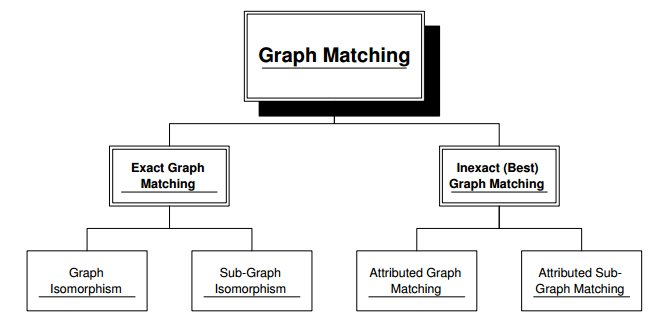
\includegraphics[width=15cm]{figures/graph_matching.jpg}
\caption{Typy graph matchingu}
\label{fig:graph_matching}
\end{center}
\end{figure}
 
 
 \section{Vytvořený algoritmus rozpoznávání operací}
 
 \subsection{Návrh ze studia článků}
 
 Vzhledem k obecné použitelnosti algoritmů pro graph matching nebyly tyto
 algoritmy shledány za vhodné k použití pro problém hledání sady
 aplikačních operací. První 3 popsané algoritmy model matchingu ( 1
 párování podle statického identifikátoru, 2. signature based matching, 3.
 similarity based matching) nejsou taktéž vhodné k použití z důdodu, že k
 rozpoznání popsaných expanzivních a reduktivních operací je nutné rozpoznat 2
 třídy, které se mapují na jednu třídu pro reduktivní operace a naopak jednu
 operaci, která se mapuje na 2 třídy. Problém rozpoznávání operací je tudíž
 nadskupinou problému model matchingu, protože matching páruje 1 ku jedné, ale
 ná na algoritmus řešící rozpoznávání operací musí řešit matching M entit ku N entitám.
 
 Zmiňované algoritmy mě inspirovaly k vytvoření Custom language specific
 matching algoritmu pro tento problém, který si z zmiňovaných algoritmů bere
 hlavně poznámku u UMLDiffu - ze všech praktických důvodů považujeme třídy se
 stejným jménem jako matchující.

 \subsection{Implementace}
 Vzniklo několik implementací párovacích algoritmů. První a nejjednodušší
 používá párování tříd podle jména, následné rozdíly řeší rozpoznáním
 konstruktivních a destruktivnívh, případně některých operací modifikačních, ať
 už tyto operace pracovali s třídami nebo s property.
 
 Složitější implementace algoritmu bylo páruje stejně jako jednodušší v
 první fázi shodné elementy - modely se mění, ale některé třídy jsou zachovány.
Shodné elementy potom tvoří jakési pilíře pro operace konstruktivní a
destruktivní, které se vážou na rozpoznané páry. Závislost rozpoznání

Algoritmus rozpoznávání operací byl napsán se snahou o zachovávání co největšího
množství dat. Ačkoliv triviální algoritmus pro přechod z modelu A k modelu B by
mohl pomocí subtraktivních operací zničit model A a následně složit model B
pomocí aditivních operací je zřejmé, že tento algoritmus neuchová žádná data.
Proto byly zavedeny Konstruktivní a destruktivní operace. 

\section{alternativní algoritmus}

V ranné fázi byl napsán prototyp jiného rozpoznávacího algoritmu, který se snaží 
minimalizovat vzdálenost současného modelu od modelu cílového pomocí rozpoznáná 
operací a aplikace operací. Výhodou tohoto přístupu je nalezení více alternativních 
cest, nevýhodou je potom velikost stavového prostoru. Algoritmus prochází těmito fázemi:

Spočítání vzdálenosti vstupního modelu od modelu cílového
Nastavení nalezeného maxima na nula
Pro každou operaci O
     zjištění, jestli má operace vhodné kandidáty na parametr
     nalezení nejvhodnějších parametrů operace



% *****************************************************************************
\chapter{Popis problému, specifikace cíle}
Tato diplomová práce si klade za cíl dokončit vývoj na projektu Migdb. Tj
doimplementovat a otestovat ORM transformace vzniklé v předešlých fázích
projektu, upravit a otestovat generátor SQL, případně upravit aplikační a
databázový metamodel.

Dalším cílem, který jsem si před vypracováním diplomové práce stanovil bylo
vytvoření a zdokumentování algoritmu generující z dvou vstupních modelů
sekvenci operací, jejichž aplikací se model zdrojový transformuje na model
koncový.

\chapter{Testování projektu Migdb}\label{chapt:testování}

V průběhu vývoje byl za účelem ověření správné funkcionality vytvořen projekt
Migdb.testing.run, který spouští jednotlivé testy kompoment aplikace. 

V rámci projektu byly vytvořeny testy komponent Workflow obsažené v packagi
migdb.testing.components.run, testy aplikační evoluce inkludované do Workflow
test\_app\_atomic.mwe2 v packagi migdb.testing.app.atomic.run, testy databázové
evoluce obsažené workflow test\_rdb\_atomic.mwe2 v packagi
migdb.testing.rdb.atomic.run, testy validátorů aplikačního a databázového
modelu obsažené v packagi migdb.testing.validators.run, test ORM transformace
struktury aplikace na DB schema + ORMo transformace obsažené v workflow
migdb.testing.orm.run, testy generování SQL schématu obsažené v packagi
migdb.testing.generators.run, integrované testy celého frameworku migdb
obsažené v packagi migdb.testing.migdb\_executer a posledními testy jsou testy
algoritmů rozpoznávajících operace obsažené v packagi
migdb.testing.app.oracle.run.

Testy komponent testují správnou funkcionalitu komponenty Comparator, která
musí správně porovnat očekávaný a reálný výstupní soubor xmi ostatních testů.
Tyto testy jsou rozděleny do více workflow, protože některé musí být neúspěšné,
jak už napovídá klíčové slovo fail v jejich názvu. Dalšími komponentami
vzniklými v rámci projektu Migdb byly QVTOExecutor, TestWorkflow,
DirectoryCleaner a TestComponent. Komponenta TestComponent vznikla, aby bylo
přehlednější a efektivnější psát QVT testy Migdb, je složena z několika dalších
načítacích, ukládacích a porovnávacích komponent a zkracuje zápis testů ve
workflow asi 10 krát. Nebylo jasné, jak vytvořit testy na správnou funkcionalitu
ostatních komponent - správné jejich zapojení do jiných testů bylo pro nás
dostatečným testem.

Ostatní testy se řadí do xmi kategorie testů, tj testů, které mají jako
vstupní model xmi soubor. Po spuštění xmi testů se v projektu
migdb.testing.run vygeneruje složka output-tests, která obsahuje výstupní data 
jednotlivých testů. Výstupní data mohou obsahovat výstupní xmi soubory
porovnávané s očekávaným xmi souborem nebo SQL souborem, který je možné
aplikovat na databázi Postgresql.

Speciálním testem je test\_code\_generator.mwe2, tento test vygeneruje pro
zadaný vstupní aplikační model a sadu aplikačních operací výstupní rdb model, sadu
databázových operací, výstupní SQL generující strukturu databáze a SQL
reprezentující výstupní databázové operace. Kromě těchto vygenerovaných dat je
možné najít ke každému testu v adresáři test\_data reálná data, s kterými může
být test spuštěn. Reálná data jsou vytvořena jen pro testy komplexnějších
operací(007 - 010), které jen nemění strukturu databáze, ale i manipulují s
daty. Postup testování tohoto testu je - spuštění workflow vedoucí k
vygenerování SQL db schematu a SQL db operací. Spuštění SQL vytvářející
strukturu databáze, spuštění SQL s daty uloženými v souboru data.sql z
přidružené složky v adresáři test\_data, aplikace vygenerovaného souboru
transformačních SQL, zobrazení výstupních dat za pomoci souboru
check\_selects.sql ze složky s daty. Bohužel nebyl nalezen lepší způsob
otestování než manuální spuštění a vizuální porovnáných selectů s očekávaným
výstupem po apliaci dané operace na data.sql.

\chapter{Ukázka zdrojového kódu práce}

%\begin{itemize}
%\item Popis řešeného problému, vymezení cílů DP/BP a požadavků na
% implementovaný systém.
%\item Popis struktury DP/BP ve vztahu k vytyčeným cílům.
%\item Rešeršní zpracování existujících implementací, pokud jsou známy.
%\end{itemize}

%*****************************************************************************
%\chapter{UML diagramy}
%\textbf{\large Tato příloha není povinná a zřejmě se neobjeví v každé práci.
% Máte-li ale větší množství podobných diagramů popisujících systém, není nutné všechny umísťovat do hlavního textu, zvláště pokud by to snižovalo jeho čitelnost.}

%*****************************************************************************
%\chapter{Instalační a uživatelská příručka}
%\textbf{\large Tato příloha velmi žádoucí zejména u softwarových
% implementačních prací.}

%*****************************************************************************
\chapter{Obsah přiloženého CD}
%\textbf{\large Tato příloha je povinná pro každou práci. Každá práce musí totiž
% obsahovat přiložené CD. Viz dále.}

%Může vypadat například takto. Váš seznam samozřejmě bude odpovídat typu vaší
%práce. (viz \cite{infodp}):

\begin{figure}[h]
\begin{center}
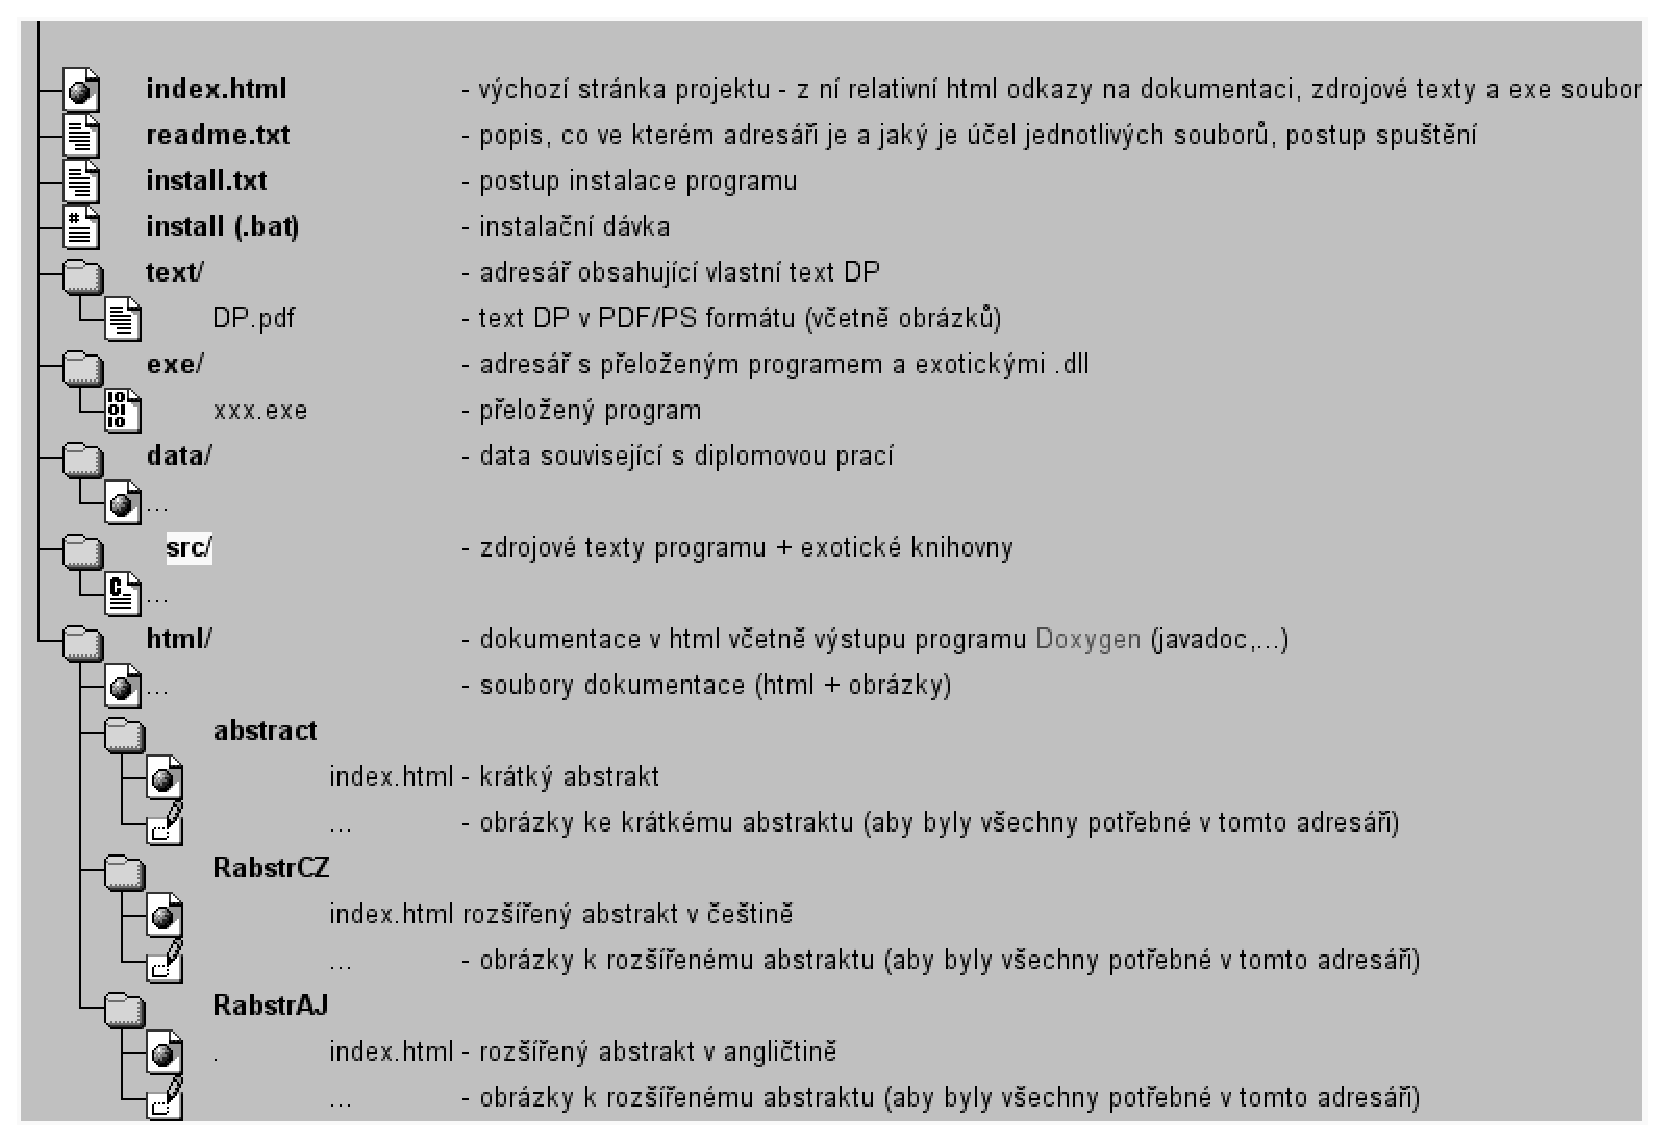
\includegraphics[width=14cm]{figures/seznamcd}
\caption{Seznam přiloženého CD}
\label{fig:seznamcd}
\end{center}
\end{figure}

\chapter{Závěr}
Po několikaletém teoretickém a praktickém studiu změn v aplikačním modelu a
jejich projevu v modelu aplikačním se nám podařilo definovat ucelenou množinu
operací, pomocí nichž je možné měnit aplikační model a definovat jejich mapování
na operace databázové úrovně.

Nejjednodušším a teoreticky nejzajímavějším tématem našeho projektu je aplikační
model, kterému byly věnovány celkově 2 bakalářké a 2 diplomové práce
BP - \cite{Tarant_bp} a  \cite{Lukes}, DP \cite{Tarant_dip},  a \cite{Mazanec}.

Implementačně nejnáročnějším a zároveň nejvíce teoreticky vyčerpaným tématem se
stala samotná transformace aplikačních operací na operace databázové, čehož jsem
využil a k implementaci, otestování a dospecifikaci tohoto mapování jsem přidal
téma čerstvé a velmi málo prozkoumané. Tímto atraktivním tématem vzhledem k
verzování modelů je automatické rozpoznávání operací provedených nad aplikačním
modelem.

Mrzí mně, že jsem se nemohl více věnovat tématu rozpoznávání operací nad
aplikačním modelem, takže jsem se nedostal k tématům jako je sémantickém
rozpoznávání operací vycházející pravděpodobně z idei sémantického
webu a implementací Resource Description Framework (RDF) a Ontology Web
Language (OWL). Implementace sémantického rozpoznávání by mohla v budoucnu
odhadnout změny nejen na základě syntaxe(struktury) databáze, ale i na základě
významu názvů jednotlivých entit v databázi. Předpokládám, že potom by bylo
možné detekovat mnohem jednoznačněji přejmenování entit - pokud by pomocí nějaké
ontologie či podobného nástroje bylo jasně specifikováno, že zvíře je nadtypem
býložravce a tento je nadtypem entity zebra, potom pokud v původním modelu
existuje třída Zebra, která má jako rodičovskou třídu nastavenu třídu
Býložravec a v výsledném modelu existuje třída Zebra s nadtřídou Zvíře a
neexistuje třída Býložravec, potom by algoritmus měl snadněji detekovat
přejmenování třídy Býložravec na třídu Zvíře i přes velkou strukturální
podobnost s jinou třídou.

Je otázkou, jak by sémantičtější rozpoznávání operací bylo prospěšné v
kontextu stále větších informačních systémech, kdy je občas těžké nazvat
smysluplně entity aplikačního modelu, natož sémantiku jejich relace vůči jiným
entitám.

V průběhu psaní této diplomové práce jsem si uvědomil, proč pro nás bylo občas
obtížné definovat správné mapování aplikačních operací na operace databázové.
Čím blíže bylo zaměření daného participanta bližší aplikačnímu modelu, tím více
si tento participant přibližoval databázový model aplikačnímu a vznikaly tak
entity jako jsou HasNoInstance s názvem rodičovské tabulky bez jakékoliv relace
rodičovství existující v databázovém modelu. Druhou chybou, kterou jsme
dělali při zaměření se na aplikační metamodel bylo modelování aplikačních
operací, které měly přespříliš složité mapování na databázové operace či někdy
až nesmyslný vliv na data v modelu - příkladem bylo modelování operace
SetOpposite, která v aplikačním modelu spojí dvě existující property tříd a až
při implementaci mapování na databázové operace bylo zjišťěno, že tato operace
pozbývá smyslu. Tato odlehlost členů Migdb od databázového modelu vytvořila
nemalé koncepční problémy, jejichž řešení bylo nutné s nemalým úsilím vymyslet
a implementovat ve velmi pozdní fázi projektu. Pokud bych psal Migdb znovu od
začátku, zaměřil bych se více na kooperaci jednotlivých částí, aby bylo pro mně
psaní transformace ORMo snazší. Tato transformace je esenciální pro chod
projektu a proto je její správná implementace alfa omegou na úspěch projektu.

Věcí, kterou bych udělal znovu jinak při psaní Migdb od začátku by bylo využití
jiného jazyka než je QVT. Tento mapovací jazyk se našim potřebám hodil málo,
proto jsme časem přestali používat jeho zakladní koncept - mapování a nahradili
ho Java-like programovacím stylem queries a helperů. Naráželi jsme na stále
větší problémy a QVT nám nepřinášelo moc užitku, nýbrž některé nevýhody. Jedna z
těchto nevýhod je například automatické ukládání jakýchkoliv pomocných entit do
výstupních modelů, které bylo nutné vyřešit (za účelem správného
otestování) speciální transformací kopírující jen ty části výstupního modelu,
které byly opravdovým výstupem, nikoliv meziproduktem. Tato transformace
vzhledem ke svojí povaze samozřejmě zpomaluje exekuci Migdb Workflow.

Poslední otázkou, na kterou jsem neměl moc času hledat odpověď je portabilita
projektu Migdb funkčního nad relační databází Postgresql na jiné
relační databáze. Předpokládám, že by nebylo složité změnit generátor kódu
pro jiné relační databáze - algoritmus vygenerování SQL kódu je poměrně
přímočarý a pro Postgresql nebyl dlouhý. Struktura jiných relačních databází
není vždy stejná, ale většinově se shoduje, takže ani modifikace databázového
metamodelu by neměla být obtížná. Moje minimální zkoumání tohoto tématu
odhalilo, že námi používaná databáze Postgresql má maximální délku 64 znaků, 
databáze Oracle má maximální délku identifikátoru 30 znaků a databáze Microsoft 
SQL server má maximum stanoveno na 128 znaků. Z tohoto vyplývá, že převod Migdb 
na databázi Microsoft SQL server by nebyl tolik problematický z tohoto pohledu.
30 znaků pro Oracle nevypadá jako problematické - vývojáři mají málokdy třídy
ukládané do databáze s jmény delšími než 30 znaků, problém nastává při zahrnutí
service pro získávání názvů databázových entit k entitám z aplikačního modelu.
Získání názvu cizího klíče, kolekce a asociační tabulky spojuje název atributu a
tabulky s nějakým prefixem a odděluje tyto položky jména podtržítky. 

Tudíž skutečné omezení délky názvu třídy může být základních 30 oslabeno o 3
(prefix FK či kolekce), oslabeno o 3 (podtržítka oddělující jednotlivé tři
části jména - prefix a dvě tabulky) děleno 2 (dvě části). Aplikací těchto
operací dostaneme horní hranici 12 znaků, která vypadá jako dostatečná, ačkoliv 
ne tolik komfortní. V této hranici jsme nicméně nezapočítaly Camel-podtržítkovou
konverzi velkých písmen na malá předražená podtržítky. Předpokládejme, že každý
identifikátor nebude mít víc jak 3 slova, tudíž musíme odečíst další 3 znaky. 9
nemusí být vždy dostatečná hranice vzhledem k velikosti nynějších systémů a
nezapočítáváme do toho fakt, že třídy v aplikačním modelu mohou(a často jsou)
prefixovány nějakým workspacem či balíčkem. Tudíž délka 9 nemusí být maximální
horní hranice jmen našich tříd a property. Je tedy zřejmé, že potom bude muset
uživatel projektu Migdb nad databází Oracle používat krátké a naprosto
neintuitivní názvy entit typu Vec102 či je nutné vymyslet jiný způsob překládání
jmen do databázového modelu, který bude automatizovaný, jednoznačný, nezávislý
na ostatních entitách v modelu a nejlépe pro člověka snadno získatelný bez
pomoci nějakého překladače.

Není možné generovat zkrátit názvy entit - vedlo by to u kolizních názvů pomocí
indexace, protože bez dalších pravidel jako například očív případě potřeby
odstranit Constraint není možné zjistit, ke které entitě

\section{Další poznámky}
\subsection{České uvozovky}
V souboru \verb|k336_thesis_macros.tex| je příkaz \verb|\uv{}| pro sázení českých uvozovek. \uv{Text uzavřený do českých uvozovek.}

% JZ: 3.5.2009 \chapter z book zajistí automaticky
%\subsection{Začátky kapitol na liché stránky}
%Ve výsledném textu je dobré, když každá kapitola začíná na liché stránce. Tedy použijte:
%\begin{verbatim}
%  \cleardoublepage\include{1_uvod}
%  \cleardoublepage\include{2_teorie}
%   atd.\ldots{}
%\end{verbatim}

%*****************************************************************************
\chapter{Seznam použitých zkratek}

\begin{description}
\item[IDE] Integrated Development Environment
\item[ORM] Object-relational mapping
\item[EMF] Eclipse modeling framework
\end{description}
\vdots

%*****************************************************************************
\chapter{UML diagramy}
\textbf{\large Tato příloha není povinná a zřejmě se neobjeví v každé práci. Máte-li ale větší množství podobných diagramů popisujících systém, není nutné všechny umísťovat do hlavního textu, zvláště pokud by to snižovalo jeho čitelnost.}

%*****************************************************************************
\chapter{Instalační a uživatelská příručka}
\textbf{\large Tato příloha velmi žádoucí zejména u softwarových implementačních prací.}

%*****************************************************************************
\chapter{Obsah přiloženého CD}
\textbf{\large Tato příloha je povinná pro každou práci. Každá práce musí totiž obsahovat přiložené CD. Viz dále.}

Může vypadat například takto. Váš seznam samozřejmě bude odpovídat typu vaší práce. 

\begin{figure}[h]
\begin{center}
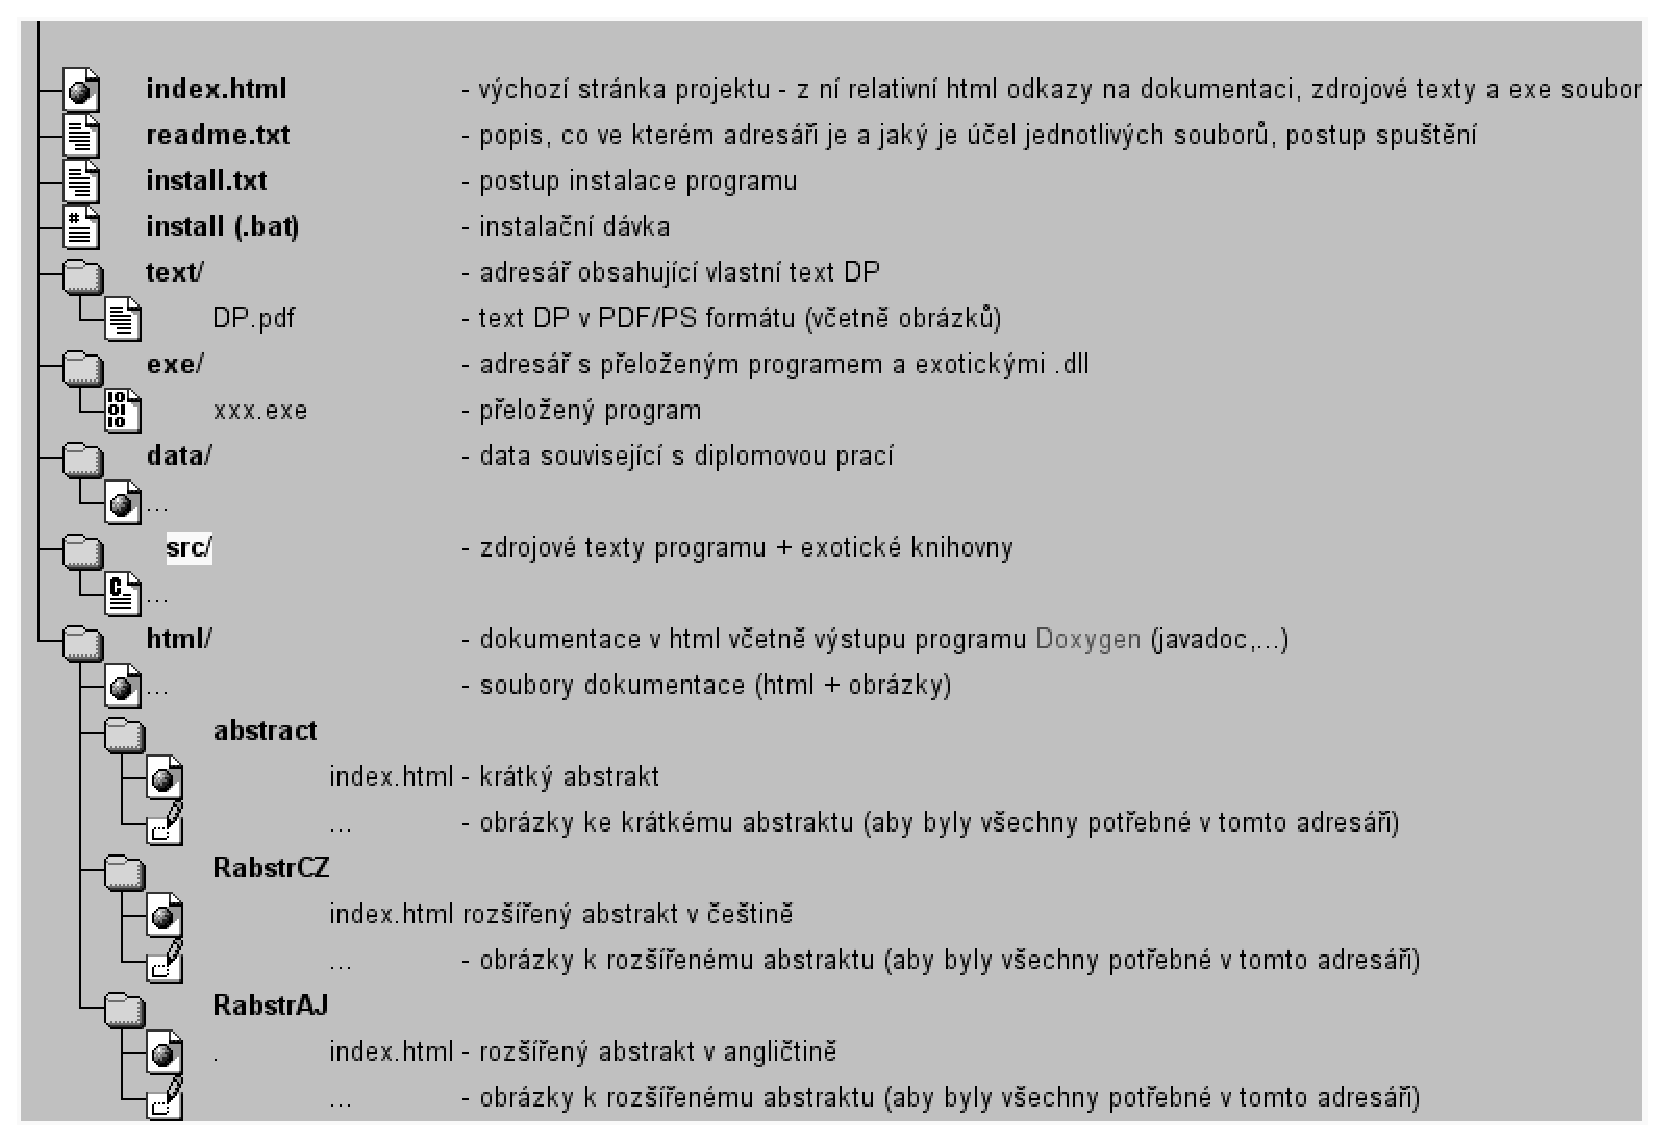
\includegraphics[width=14cm]{figures/seznamcd}
\caption{Seznam přiloženého CD --- příklad}
\label{fig:seznamcd}
\end{center}
\end{figure}

Na GNU/Linuxu si strukturu přiloženého CD můžete snadno vyrobit příkazem:\\ 
\verb|$ tree . >tree.txt|\\
Ve vzniklém souboru pak stačí pouze doplnit komentáře.

Z \textbf{README.TXT} (případne index.html apod.)  musí být rovněž zřejmé, jak programy instalovat, spouštět a jaké požadavky mají tyto programy na hardware.

Adresář \textbf{text}  musí obsahovat soubor s vlastním textem práce v PDF nebo PS formátu, který bude později použit pro prezentaci diplomové práce na WWW.
 \bibliographystyle{alpha}
\bibliography{reference}

\end{document}
